\documentclass[onecolumn, draftclsnofoot,10pt, compsoc]{IEEEtran}
\usepackage[usenames, dvipsnames]{color}
\usepackage{graphicx}
\usepackage[section]{placeins}
\usepackage{url}
\usepackage{setspace}

%For indentItem command
\usepackage{enumitem}
\usepackage{changepage}

%For \textrightarrow
\usepackage{textcomp}
\usepackage{tgpagella}

%For Gantt Chart
\usepackage{xspace}
\usepackage{pgfgantt}
\usepackage{subcaption}

\usepackage{alltt}
\usepackage{float}
\usepackage{color}
\usepackage{url}

\usepackage{geometry}
\geometry{textheight=9.5in, textwidth=7in}
\setlength\parindent{0pt}

\usepackage{tabu}
\usepackage{longtable}

\usepackage{xspace}
\usepackage{pgfgantt}
\usepackage{subcaption}
\usepackage{graphicx}
\usepackage{color}
\usepackage{xcolor,pifont}

\usepackage[utf8]{inputenc}
\usepackage[english]{babel}


\newcommand{\newpara}{\\[0.1in]}

\newcommand{\greencheck}{\textcolor{ForestGreen}{\ding{51}}}%
\newcommand{\redcheck}{\textcolor{red}{\ding{51}}}%


% 1. Fill in these details
\def \CapstoneTeamName{\textbf{Insert Team Name Here} }
\def \CapstoneTeamNumber{8}
\def \botname{Kora\xspace}
\def \GroupMemberOne{Austin Row}
\def \GroupMemberTwo{Jeremy Fischer}
\def \CapstoneProjectName{\botname}
\def \CapstoneSponsorCompany{Autodesk}
\def \CapstoneSponsorPerson{Anand Karyekar \& Jennifer Talaga}

\def \speechToText{Wit.ai\xspace}



% 2. Uncomment the appropriate line below so that the document type works
\def \DocType{ Final Report}

\newenvironment{indentItem}[1][1cm]{\begin{adjustwidth}{#1}{}}{\end{adjustwidth}}
\newcommand{\designConcernDef}[3]{
    \subsubsection{#1}\label{#1}
        \begin{tabular}[t]{r p{6in}}
            Stakeholder(s): & #2 \\
            Concern: & #3 \\
        \end{tabular}
}
\newcommand{\designConcernRef}[1]{
    #1 (defined in section \ref{#1})
}
\newcommand{\designElementDef}[4]{
    \subsubsection{#1}\label{#1}
        \begin{tabular}[t]{r p{6in}}
            Type: & #2 \\
            Purpose: & #3 \\
            Author: & #4 \\
        \end{tabular}
}
\newcommand{\designElementRef}[1]{
    \subsubsection{#1}
        See section \ref{#1} for element definition.
}
\newcommand{\NameSigPair}[1]{\par
\makebox[2.75in][r]{#1} \hfil 	\makebox[3.25in]{\makebox[2.25in]{\hrulefill} \hfill		\makebox[.75in]{\hrulefill}}
\par\vspace{-12pt} \textit{\tiny\noindent
\makebox[2.75in]{} \hfil		\makebox[3.25in]{\makebox[2.25in][r]{Signature} \hfill	\makebox[.75in][r]{Date}}}}
% 3. If the document is not to be signed, uncomment the RENEWcommand below
\renewcommand{\NameSigPair}[1]{#1}

%%%%%%%%%%%%%%%%%%%%%%%%%%%%%%%%%%%%%%%
\graphicspath {{Photos/}}

\begin{document}
\begin{titlepage}
    \pagenumbering{gobble}
    \begin{singlespace}
    	
\includegraphics[height=4cm]{coe_v_spot1}
        %\hfill
        % 4. If you have a logo, use this includegraphics command to put it on the coversheet.
        \par\vspace{.2in}
        \centering
        \scshape{
            \huge CS Capstone \DocType \par
            {\large\today}\par
            \vspace{.5in}
            \textbf{\Huge\CapstoneProjectName}\par
            \vfill
            {\large Prepared for}\par
            \Huge \CapstoneSponsorCompany\par
            \vspace{5pt}
            {\Large\NameSigPair{\CapstoneSponsorPerson}\par}
            {\large Prepared by }\par
            % 5. comment out the line below this one if you do not wish to name your team
            %\CapstoneTeamName\par
            \vspace{5pt}
            {\Large
                \NameSigPair{\GroupMemberOne}\par
                \NameSigPair{\GroupMemberTwo}\par
            }
            \vspace{20pt}
        }
        \begin{abstract}

        \end{abstract}
    \end{singlespace}
\end{titlepage}
\newpage
\pagenumbering{arabic}
\tableofcontents
% 7. uncomment this (if applicable). Consider adding a page break.
%\listoffigures
%\listoftables
\clearpage




















%	Who requested it?
%	Why was it requested?
%	What is its importance?
%	Who was/were your client(s)?
%	Who are the members of your team?
%	What were their roles?
%	What was the role of the client(s)? (I.e., did they supervise only, or did they participate in doing development)

\section{Introduction to Project}
	Kora was requested by Patti Vrobel on behalf of Autodesk.
	After Fall term the project was passed on to Anand Karyekar and Jennifer Talaga, who supervised the project.
	\newpara
	Since the inception of publicly available computers until around 2006 society has interacted with computers in the same manner – keyboard and mouse.
	Recently there’s been a moving trend toward making computers and machines more interactive.
	Nintendo launched the Wii in 2006 and Microsoft’s XBOX division followed in 2010 with the Kinect \cite{wii}\cite{kinect}.
	 Apple launched Siri in 2010 and Microsoft and Google followed shortly after with their smart assistants \cite{siri}.
	 Autodesk realizes the competitive advantage of having their products more interactive.
	 This is what lead to Kora.
	\newpara
	Autodesk has the opportunity to gain much more from making their products more interactive than simply retaining and attracting users due to the new ease of use.
	From a business perspective, enabling natural language processing allows for a new addition to user data that is rich in potential!
	Instead of only collecting button clicks on dropdown menus and ribbon items, with a voice interface Autodesk would be able to collect exactly what the user is intending to do.
	This form of data collection rips away the ambiguity of the data.
	\newpara
	Kora was created by Austin Row and Jeremy Fischer.
	Since the team consisted of just the two of us, we didn't have assigned roles.
	Instead, we both touched all aspects of the project.













\section{Requirements Document}

	\subsection{Introduction}
	The introduction outlines the purpose and scope of the project.
	This section is also responsible for defining any prerequisite acronyms and terms used in the document.
	\subsubsection{Purpose}
	The purpose of this document is to specify the exact requirements that \botname must meet to be considered a successful project.
	This document is a mutual agreement between the client and developers regarding the expected result of this project.
	The intended audience is the two aforementioned parties.
	\subsubsection{Scope}
	\botname will be a speech-based virtual assistant for Fusion that lets users perform any one of a subset of tasks within the product, such as rotating the camera or extruding a face, by verbally instructing it to perform the task.
	Workflows in Fusion that are not suited for handling by a voice interface will not be supported by \botname.
	As a stretch goal, \botname will be capable of questioning the user and using responses to predict and automatically assist with future user behavior.
	It will be a plugin that is bundled with Fusion and will be part of the product's standard download.

	\botname will offer users a tool that decreases the time required to achieve their goals within Fusion by offering an interface that runs in parallel with and complements the keyboard and mouse.
	If the stretch goal is achieved, \botname will further increase productivity by learning to predict and automate specific workflows within the product.


	\subsubsection{Definitions, Acronyms, and Abbreviations}
	\begin{table}[h]
		\centering
		\caption{Definitions}
		\label{my-label}
		\begin{tabular}{|l|l|}
			\hline
			\textbf{Term} & \textbf{Definition} \\ \hline
			\botname & The virtual assistant that is the focus of this project \\ \hline
			NLP & Natural Language Processing \\ \hline
			API & Application Programing Interface \\ \hline
			CAD & Computer Aided Design \\ \hline
			CAM & Computer Aided Manufacturing \\ \hline
			Fusion & An Autodesk Cloud-based 3D CAD/CAM tool/product \\ \hline
			Task & In the context of Fusion, a function or operation that can be performed in Fusion \\ \hline
			Plugin & Software that adds specific new functionlity to another piece of software \\ \hline
			User & A person that interacts with \botname or Fusion depending on the context \\ \hline
			Workflow & A sequence of related tasks \\ \hline
		\end{tabular}
	\end{table}
	\subsubsection{Overview}
	%This section describes the contents and organization of the rest of the document.
	The rest of this document outlines intended uses and specific functionalities of \botname as well as assumptions, dependencies, and constraints that pertain to the project.

	\subsection{Overall Description}
	\subsubsection{Product Perspective}

	\subsubsection{User Interfaces}
	The user will interact with \botname via voice commands given in English.
	%To initiate a command, the user will say "\botname" followed by the command.
	To initiate \botname, the user will press the "Activate" button on the Add-Ins drop down in Fusion.

	As part of a stretch goal, \botname will periodically ask questions back to the user via a speech synthesizer.

	\subsubsection{Hardware Interfaces}
	\botname will be supported on desktop and laptop computers that support Fusion and have microphones to receive the user's speech.
	For stretch goal support, devices will also need speakers through which \botname can speak back to the user.

	\subsubsection{Software Interfaces}
	\botname needs to translate supported speech commands received from the user to the equivalent tasks within the user's Fusion project.
	For this, a series of open source NLP projects will be linked to derive meaning from speech.
	The derived meaning will then be mapped to a Fusion API call.

	\subsubsection{Site Adaptation Requirements}
	Since \botname interacts with Fusion using existing architecture, Fusion will not need to be modified to support it.

	\subsubsection{Product Functions}
	\botname will allow the user to perform tasks in Fusion via a voice interface.
	Each voice command given by the user will be mapped to a specific task which will then be performed in the open Fusion project.

	As a stretch goal, \botname will periodically ask the user questions regarding why they have performed specific tasks.
	The questions asked by \botname will pertain to specific predefined contexts.
	\botname will record user responses and save a transcript along with contextual information.
	Responses will also be used to try to predict and assist with future user actions.

	All interactions with \botname will be logged for debugging and future development purposes.

	\subsubsection{User Characteristics}
	\botname will have two types of users: administrators and designers.
	Administrators will have access to data collected by \botname including the command logs and, if the stretch goal is accomplished, user responses to questions from \botname.

	The primary user is the designer who is working on projects inside of Fusion.
	Due to the technical knowledge needed to work within Fusion, it can be assumed that designers are technically oriented.
	However, no extra knowledge outside of that needed to operate Fusion will be needed to operate \botname.

	\subsubsection{Constraints}
	\botname will not be integrated with the Fusion source code and thus will be constrained in what tasks it can perform by what is offered in the Fusion API.

	\subsubsection{Assumptions and Dependencies}
	Since this project does not focus on developing software to handle speech recognition and natural language processing, it depends on the existence of adequate open source resources for handling this aspect of \botname.

	The stretch goal assumes that the Fusion API offers a way to view actions that the user performs with their keyboard and mouse.
	Without this capability, the application's knowledge of user actions will be limited to the actions that the user performs through \botname.

	\subsection{Specific Requirements}
	\subsubsection{External Interface}
	 After \botname is released, Fusion users will be shown a modal the next time that they log into the product that gives a brief description of \botname and asks if they would like to enable it.
	If a user chooses not to enable \botname, their Fusion editor environment will not be changed.

	Users that enable \botname will be presented with an onboarding process that incorporates an interactive demo.
	The onboarding process will start with a popup that introduces \botname with a concise description of its purpose.
	The user will then be able to click "Next" to transition to an interactive demo.
	The interactive demo will consist of several sequential popups that each ask the user to tell \botname to perform a specific command.
	This will make the user aware of \botname and the functionality that it offers.

	\subsubsection{Functional Requirements}
	This section includes the requirements that specify all the fundamental actions of the software system.
	\subsubsection{Functional Requirement 1}
	TITLE: Status Messaging \\
	DESCRIPTION: The system shall alert the user when it has understood a command as well as when it has failed to interpret a user command or has reached an error state. \\
	RATIONALE: This clarifies for the user if \botname is doing what they think it should be doing or if they need to try again.

	\subsubsection{Functional Requirement 2}
	TITLE: Extrude \\
	DESCRIPTION: \botname shall be able to extrude a selected face. \\
	RATIONALE: This is a task that users perform often.

	\subsubsection{Functional Requirement 3}
	TITLE: Rotate Camera \\
	DESCRIPTION: \botname shall be able to rotate the Fusion camera. \\
	RATIONALE: This is a task that users perform often.

	\subsubsection{Functional Requirement 4}
	TITLE: Save Project \\
	DESCRIPTION: \botname shall be able to save a Fusion project. \\
	RATIONALE: This is a task that users perform often.

	\subsubsection{Functional Requirement 5}
	TITLE: Logging User Interactions \\
	DESCRIPTION: \botname shall log every interaction that a user has with it and the result of that interaction. \\
	RATIONALE: This offers helpful information for debugging purposes. This information can also be used to learn how \botname is being used and to drive future development.

	\subsubsection{Functional Requirement 6}
	TITLE: Command Signaling \\
	DESCRIPTION: \botname will begin listening for a command after hearing the user say "\botname". \\
	RATIONALE: This is a pattern that is used in many successful voice assistants to signal when to start listening for a command.

	%	%
	%	Below are stretch goals
	%	%

	\subsubsection{Stretch Functional Requirement 1}
	TITLE: Smart Assistant \\
	DESCRIPTION: \botname will be able to offer executable suggestions in the form of "Would you like to...?" questions that the user will respond in the affirmative to at least 15\% of the time. \\
	RATIONALE: This is the ultimate vision for \botname in which it can predict what the user will want to do next and will be able to perform those next steps for the user.

	\subsubsection{Performance Requirements}
	The section lists the performance requirements that will be met by \botname.

	\subsubsection{Performance Requirement 1}
	TITLE: Response Time \\
	DESCRIPTION: It will take a user at most one second longer to perform a supported task through \botname than it would take when using a keyboard and mouse. \\
	RATIONALE: The user must feel that \botname enhances rather than slows their development speed.

	\subsubsection{Design Constraints}
	\botname will execute tasks in Fusion via the Fusion API.
	Therefore supported tasks will constrained to those capable of being performed by the API.

	\subsection{Release Plan}

	\subsubsection{Release plan}
	\begin{figure}[H]
		\begin{center}
			%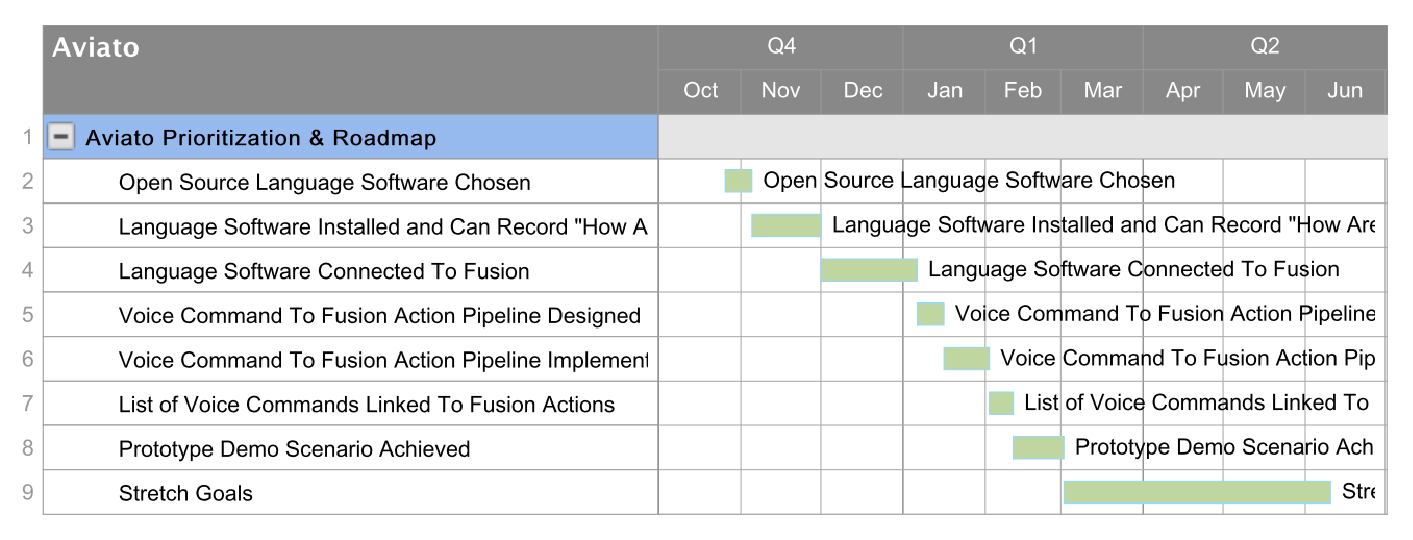
\includegraphics[width=1\textwidth]{ganttChart.eps}
			%Changed Gantt chart to be modifiable.
			\begin{ganttchart}[
				y unit title=0.4cm,
				y unit chart=0.5cm,
				vgrid,
				hgrid,
				title left shift=.05,
				title right shift=.05,
				title height=1,
				group right shift=0
				]{1}{28}
				\gantttitle{Months}{28} \\
				\gantttitle{October}{4}
				\gantttitle{November}{4}
				\gantttitle{December}{4}
				\gantttitle{January}{4}
				\gantttitle{February}{4}
				\gantttitle{March}{4}
				\gantttitle{April}{4} \\

				\ganttbar{Problem Statement}{1}{2} \\
				\ganttbar{Requirements Document}{3}{4} \\
				\ganttbar{Technology Review}{5}{6} \\
				\ganttbar{Design \botname}{7}{8} \\
				\ganttbar{Fall Progress Report}{9}{9} \\
				\ganttbar{Speech-to-Task Pipeline}{10}{14} \\
				\ganttbar{Create Alpha Demo}{18}{18} \\
				\ganttbar{Train NLP Modules}{13}{25} \\
				\ganttbar{Performance Testing}{16}{25} \\
				\ganttbar{Create Beta Demo}{22}{22} \\
				\ganttbar{Smart Assistant Stretch Goal}{15}{23} \\
				\ganttbar{Engineering Expo}{26}{26}

			\end{ganttchart}
			\captionsetup{justification=centering}
			\caption{\botname Development Schedule}
			\label{fig:developmentSchedule1}
		\end{center}
	\end{figure}

	\subsection{Changes}
		\subsubsection{Change History}
		\begin{table}[H]
			\centering
			\caption{Change History}
			\label{my-label}
			\begin{tabular}{|l|l|}
				\hline
				\textbf{Date}     & \textbf{Change Description}   \\ \hline
				November 16, 2017 & {First requirements document draft} \\ \hline
				May 8, 2018 & {User onboarding and Kora wake-word taken out. Performance requirement loosened.} \\ \hline
			\end{tabular}
		\end{table}

		The user onboarding requirement was taken off due to an issue on Fusion 360's end.
		To complete the onboarding through the Fusion API we needed to use Fusion palettes.
		According to the Fusion API documentation, the palettes support JavaScript. However, the sample palette given on the API's website didn't work.
		After further discussion with our clients it appears there is a problem on Fusion's end, and the team is working on it.
		Unfortunately, this meant we couldn't accomplish the onboarding requirement until the JavaScript issue was handled.
		\newpara
		The performance metric was altered from \textit{at most one second longer than the task would take manually} to \textit{at most three seconds longer than the task would take manually}.
		This was due to WIT.ai's average latency of three seconds to interpret the streamed audio.
		We could have pivoted and used a different NLP, but our clients instructed to keep working on the other requirements and come back to the latency issue if time allows.
		\newpara
		The wake-word requirement was taken out because WIT.ai didn't support a wake-word, and we didn't have enough time to incorporate an open source solution for it.
		\newpara
		We remind you at the time the requirements document was written our team had three members, and so the workload we assigned reflected that. Unfortunately, at the beginning of Kora's development our third member left the group, putting more of a workload on Austin and Jeremy's plates.

	\subsection{Final Gantt Chart}
		\begin{figure}[H]
			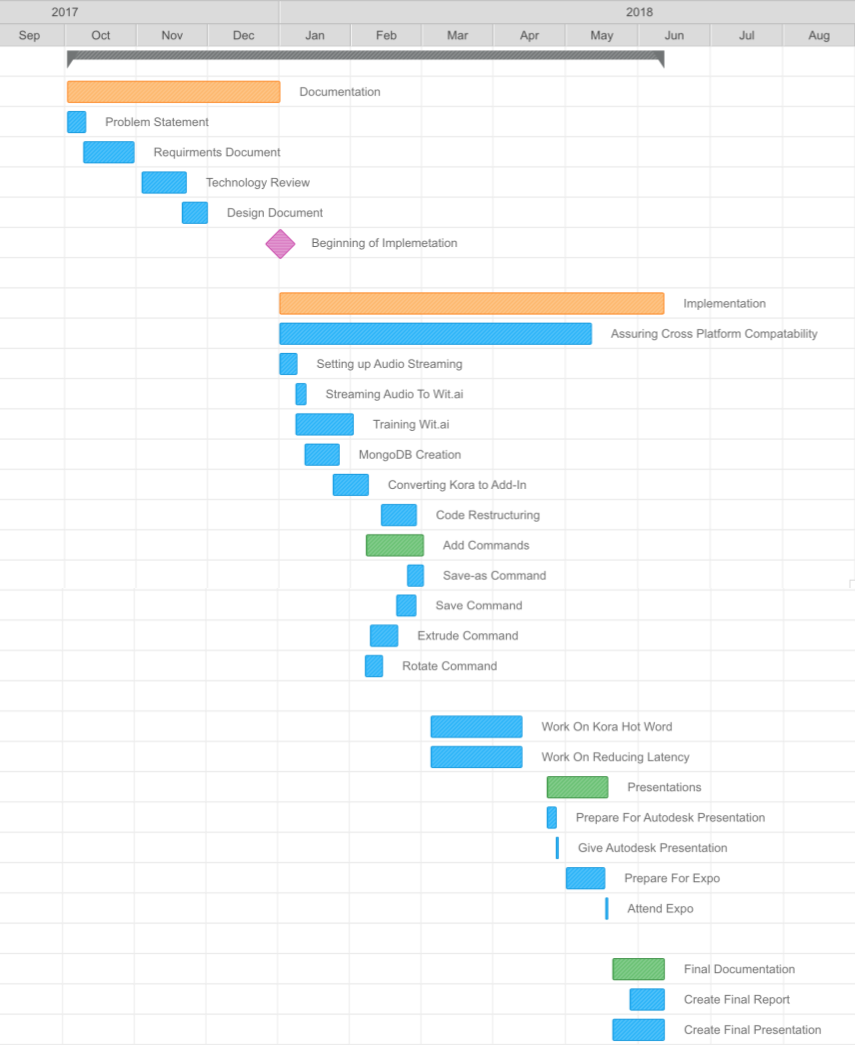
\includegraphics[width=16cm]{finalGantt.eps}
			\centering
			\caption{Kora's final Gantt chart showing a rough estimate of when Kora's components were developed.}
		\end{figure}


















\section{Design Document}
	\subsection{Document Details}
	\subsubsection{Date of Issue and Status}
	This document was issued December 1, 2017 and is the first complete iteration of the design document.

	\subsubsection{Authorship}
	Jeremy Fischer, Austin Row, and James Stallkamp are the authors of this document and the developers of \botname.

	\subsubsection{Change History}
	\begin{table}[H]
		\centering
		\caption{Change History}
		\label{my-label}
		\begin{tabular}{|l|l|}
			\hline
			\textbf{Date}     & \textbf{Change Description}   \\ \hline
			November 30, 2017 & {First design document draft} \\ \hline
			January 19, 2018 & {Module interaction diagram updated} \\ \hline
		\end{tabular}
	\end{table}

	\subsection{Introduction}
	\subsubsection{Purpose}
	The purpose of this design document is to outline how \botname's functionality will be achieved.
	More generally, this document describes how the client's requirements will be met.
	\botname's developers will use this document as a roadmap during implementation.

	\subsubsection{Scope}
	This document focuses on the relationships between \botname's components and their individual processes, and how they work together to satisfy the project's requirements.


	\subsubsection{Summary}
	\botname will be a speech-based virtual assistant for Fusion that lets users perform any one of a subset of tasks within the product, such as saving a document or opening a menu, by verbally instructing it to perform the task.
	Workflows in Fusion that are not suited for handling by a voice interface will not be supported by \botname.
	As a stretch goal, \botname will be capable of questioning the user and using responses to predict and automatically assist with future user behavior.
	This functionality will be implemented as a plugin that is bundled with Fusion and will be part of the product's standard download.
	\newpara
	\botname will offer users a tool that decreases the time required to achieve their goals within Fusion by offering an interface that runs in parallel with and complements the keyboard and mouse.
	If the stretch goal is achieved, \botname will further increase productivity by learning to predict and automate specific workflows within the product.

	\subsection{Glossary}
	\begin{table}[H]
		\centering
		\caption{Glossary}
		\label{my-label}
		\begin{tabular}{|l|l|}
			\hline
			\textbf{Term} & \textbf{Definition} \\ \hline
			\botname & The virtual assistant that is the focus of this project \\ \hline
			NLP & Natural Language Processing \\ \hline
			API & Application Programing Interface \\ \hline
			CAD & Computer Aided Design \\ \hline
			CAM & Computer Aided Manufacturing \\ \hline
			UI & User Interface \\ \hline
			Fusion & An Autodesk Cloud-based 3D CAD/CAM tool/product \\ \hline
			Task & In the context of Fusion, a function or operation that can be performed in Fusion \\ \hline
			Plugin & Software that adds specific new functionality to another piece of software \\ \hline
			User & A person that interacts with \botname or Fusion depending on the context \\ \hline
			Workflow & A sequence of related tasks \\ \hline
		\end{tabular}
	\end{table}

	\subsection{Design Stakeholders and Concerns}
	\designConcernDef{System Decomposition}{Developers}{How is the software system decomposed into components?}
	\designConcernDef{Component Functional Responsibilities}{Developers}{What functionality is each software component responsible for?}
	\designConcernDef{User-Application Interface}{Client, Developers}{What interfaces will exist for users to interact with the application and for the application to communicate with users?}
	\designConcernDef{Internal Interfaces}{Developers}{What internal interfaces will exist between software components?}
	\designConcernDef{Component Interactions}{Developers}{Which components of the software system will interact?}
	\designConcernDef{Component Interaction Responsibilities}{Developers}{What are the responsibilities of each component of the software system in the context of interactions?}
	\designConcernDef{Architecture}{Developers}{What architecture defines the software system?}
	\designConcernDef{System States}{Developers}{What are the possible states the software system can be in?}
	\designConcernDef{State Activities}{Developers}{What defines each of the states of the system?}
	\designConcernDef{State Transitions}{Developers}{When does the system transition from one state to another?}
	\designConcernDef{Log File Location}{Developers}{Where will data regarding user interactions be logged?}
	\designConcernDef{Log File Content}{Developers}{What will be stored in log files?}
	\designConcernDef{Log File Access}{Developers}{How will stored log files be accessed?}


	\subsection{Design Viewpoint: Composition}
	\subsubsection{Addressed Design Concerns}
	\begin{itemize}
		\item \designConcernRef{System Decomposition}
		\item \designConcernRef{Component Functional Responsibilities}
	\end{itemize}

	\subsubsection{Design Elements}
	\designElementDef{Master Module}
	{Module}
	{Facilitates communication between modules and manages application state.}
	{James Stallkamp}
	\designElementDef{UI Module}
	{Module}
	{Provides user a way to interact with \botname and expresses the application state to the user.}
	{James Stallkamp}
	\designElementDef{Speech-to-Intent Module}
	{Module}
	{Anaylzes speech input and produces a intent object in JSON format.}
	{James Stallkamp}
	\designElementDef{Logger Module}
	{Module}
	{Stores runtime and contextual information to be used for training \botname.}
	{James Stallkamp}
	\designElementDef{Fusion Module}
	{Module}
	{Translates intent into Fusion API commands and executes them.}
	{James Stallkamp}
	\designElementDef{Text-to-Speech Module}
	{Module}
	{Synthesizes an audio output from a given text input.}
	{James Stallkamp}
	\designElementDef{Action Prediction Module}
	{Module}
	{Trains \botname to become a more powerful assistant.}
	{James Stallkamp}

	\subsubsection{Design View: Modules}
	\botname is composed of seven primary modules.
	\subsubsection{Master Module}
	\begin{indentItem}
		The Master module is responsible for coordinating all other modules.
	\end{indentItem}
	\subsubsection{UI Module}
	\begin{indentItem}
		The UI module is responsible for all interaction with the user.
		This module will collect input and communicate it to the Master module as well output regular feedback to the user.
	\end{indentItem}
	\subsubsection{Speech-to-Intent Module}
	\begin{indentItem}
		The Speech-to-Intent module will take in audio input and output a JSON object containing information on the spoken input.
		This intent module will construct the JSON object and return it to master.
	\end{indentItem}
	\subsubsection{Logger Module}
	\begin{indentItem}
		The Logger Module will create a persist-able data object that will be loaded with run time information from \botname.
		These data objects will be analyzed and used to help train \botname for future development.
	\end{indentItem}
	\subsubsection{Fusion Module}
	\begin{indentItem}
		The next module is the Fusion module, this module will handle executing Fusion commands.
		The Fusion module will parse information from the JSON intent object to construct and execute a Fusion command.
	\end{indentItem}
	\subsubsection{Text-to-Speech Module}
	\begin{indentItem}
		In order for \botname to speak to the user it will need a voice synthesizer module.
		This module will receive text input and produce an audio output that can be played to the user.
	\end{indentItem}
	\subsubsection{Action Prediction Module}
	\begin{indentItem}
		The Action Prediction module is responsible for training \botname to recognize patterns and improve functionality.
	\end{indentItem}

	\subsection{Design Viewpoint: Information}
	\subsubsection{Addressed Design Concerns}
	\begin{itemize}
		\item \designConcernRef{Log File Location}
		\item \designConcernRef{Log File Content}
		\item \designConcernRef{Log File Access}
	\end{itemize}


	\subsubsection{Design Elements}
	\designElementDef{MongoDB}{Database}{Database to hold the log files}{Jeremy Fischer}
	\designElementDef{JSON object}{Storage structure}{The structure the information will be stored in}{Jeremy Fischer}
	\designElementDef{HTTP calls}{Access mechanism}{How the data will be posted and accessed}{Jeremy Fischer}

	\subsubsection{Design View: Contents}
	The contents of the data will be:
	\begin{itemize}
		\item the intent generated by the Speech-to-Intent module
		\item the context generated by the Speech-to-Intent module such as quantities
		\item whether the user's request was successfully processed
		\item the posting date
		\item the posting time
		\item the user identification
	\end{itemize}

	\subsubsection{Design View: Access}
	The data will be posted and accessed via HTTP calls to the database.

	\subsubsection{Design View: Structure}
	The data will be stored in a MongoDB database.
	Each entry in the database will resemble the JSON object that is returned from the Speech-to-Intent module driver method.



	\subsection{Design Viewpoint: Patterns}
	\subsubsection{Addressed Design Concerns}
	\begin{itemize}
		\item \designConcernRef{Architecture}
	\end{itemize}

	\subsubsection{Design Elements}
	\designElementDef{Mediator Design Framework}
	{System Architecture}
	{\botname has a simple mediator that coordinates all interactions between all other components.}
	{James Stallkamp}
	\subsubsection{Design View: Software Architecture}
	\botname is structured according to a mediator design pattern.
	\botname will have a Master module that coordinates interactions between itself and all other modules.
	The Master module controls \botname's flow and ensures that the correct data gets to the correct module.


	\subsection{Design Viewpoint: Interfaces}
	\subsubsection{Addressed Design Concerns}
	\begin{itemize}
		\item \designConcernRef{User-Application Interface}
		\item \designConcernRef{Internal Interfaces}
	\end{itemize}

	\subsubsection{Design Elements}
	\designElementDef{UI Module Interface}{Internal Interface}{Defines rules governing interactions with the UI module.}{Austin Row}
	\designElementDef{Speech-to-Intent Module Interface}{Internal Interface}{Defines rules governing interactions with the Speech-to-Intent module.}{Austin Row}
	\designElementDef{Logging Module Interface}{Internal Interface}{Defines rules governing interactions with the Logging module.}{Austin Row}
	\designElementDef{Text-to-Speech Module Interface}{Internal Interface}{Defines rules governing interactions with the Text-to-Speech module.}{Austin Row}
	\designElementDef{Fusion Module Interface}{Internal Interface}{Defines rules governing interactions with the Fusion module.}{Austin Row}
	\designElementDef{Action Prediction Module Interface}{Internal Interface}{Defines rules governing interactions with the Action Prediction module.}{Austin Row}
	\designElementDef{User Interface}{External Interface}{Defines rules governing how the human user can interact with \botname.}{Austin Row}
	\subsubsection{Design View: Module Interfaces}
	The various modules that compose the project each have an interface defined by functions that are unique to that module.
	Following is documentation for the functions that define the interface to each module.
	\subsubsection{UI Module Interface}
	\begin{tabular}[t]{l p{6in}}
		\hline
		Function: & notify \\
		Description: & Shows a notification to the user in the Fusion editor. \\
		Parameters: & notification -- a KoraNotification object that contains members to specify visual characteritics and content for notification that is shown to user. \\
		Return: & 1 on successful showing of notification, 0 otherwise. \\
		\hline
		Function: & listen \\
		Description: & Listens through microphone until user voice command is given then returns data about the command. \\
		Parameters: & N/A \\
		Return: & Wit.ai JSON response object with data from user command. \\
		\hline
		Function: & voicePrompt \\
		Description: & Asks user a question via a voice sythesizer and records and interprets response. \\
		Parameters: & text -- the text manuscript for the question that the user should be asked. \\
		& timeout (optional) -- the amount of time that \botname should wait for a response before giving up. \\
		Return: & Wit.ai JSON response object with data from user response. \\
		\hline
	\end{tabular}

	\subsubsection{Speech-to-Intent Module Interface}
	\begin{tabular}[t]{l p{6in}}
		\hline
		Function: &  streamAudioToWit \\
		Description: & Streams audio data to Wit.ai via provided audio stream and returns Wit.ai JSON response object. \\
		Parameters: & audioStream -- an Pyaudio input stream. \\
		Return: & Wit.ai JSON response object for streamed audio. \\
		\hline
	\end{tabular}

	\subsubsection{Logging Module Interface}
	\begin{tabular}[t]{l p{6in}}
		\hline
		Function: & debug \\
		Description: & Logs data to log file with DEBUG tag. \\
		Parameters: & message -- string with message to be logged. \\
		Return: & 1 on message successfully being added to log file, 0 otherwise. \\
		\hline
		Function: & warn \\
		Description: & Logs data to log file with WARN tag. \\
		Parameters: & message -- string with message to be logged. \\
		Return: & 1 on message successfully being added to log file, 0 otherwise. \\
		\hline
		Function: & error \\
		Description: & Logs data to log file with ERROR tag. \\
		Parameters: & message -- string with message to be logged. \\
		Return: & 1 on message successfully being added to log file, 0 otherwise. \\
		\hline
	\end{tabular}

	\subsubsection{Text-to-Speech Module Interface}
	\begin{tabular}[t]{l p{6in}}
		\hline
		Function: & textToSpeech \\
		Description: & Converts message given as text to raw audio and returns audio. \\
		Parameters: & text -- the text to be converted to audio. \\
		Return: & List object containing raw audio data for text. \\
		\hline
	\end{tabular}

	\subsubsection{Fusion Module Interface}
	\begin{tabular}[t]{l p{6in}}
		\hline
		Function: & executeCommand \\
		Description: & Uses Fusion API to execute command(s) specified in Wit.ai JSON response object passed as argument. \\
		Parameters: & command -- a Wit.ai JSON response object with data needed to interpret user's command. \\
		& callback (optional) -- a function that accepts an integer associated with a command execution status to be called at the finish of executeCommand. \\
		Return: & An integer code associated with a particular status (e.g. success, runtime failure, unrecognized command, etc.). \\
		\hline
	\end{tabular}

	\subsubsection{Action Prediction Module Interface}
	\begin{tabular}[t]{r p{6in}}
		\hline
		Function: & predict \\
		Description: & Uses a Wit.ai JSON response object to predict what user's next command will be. \\
		Parameters: & command -- a Wit.ai JSON response object with data derived from a user voice command. \\
		Return: & A JSON object containing prediction for next user voice command and unique integer ID to identify prediction. \\
		\hline
		Function: & learn \\
		Description: & Gives feedback to \botname's prediction model so that it can improve. \\
		Parameters: & predictionID -- unique integer identifier for a previous prediction made by the model. \\
		& actual -- JSON with data regarding what the user actually did after the model made its prediction. \\
		Return: & N/A \\
		\hline
	\end{tabular}

	\subsubsection{Design View: User Interface}
	The user interface can be divided into two interaction types: the user giving \botname a command and \botname replying to the user with the application status.
	There are two use patterns for a user when they give \botname a command. The first way to give a command is to say the wake word followed by the command.
	When the user says the wake word, it signals to \botname that it should be actively listening for a command.
	The other method is to click the wake button that acts as an alternative to the wake word then say the command.
	\newpara
	Through the user interface, the application responds back to the user with the status of the previous command.
	If the command succeeds, the application uses a voice synthesizer to alert the user that the previous command succeeded.
	If the command fails, the application uses the voice synthesizer to alert the user that the previous command failed.

	\subsection{Design Viewpoint: Interactions}
	\subsubsection{Addressed Design Concerns}
	\begin{itemize}
		\item \designConcernRef{Component Interactions}
		\item \designConcernRef{Component Interaction Responsibilities}
	\end{itemize}

	\subsubsection{Design Elements}
	\designElementRef{Master Module}
	\designElementRef{UI Module}
	\designElementRef{Speech-to-Intent Module}
	\designElementRef{Logger Module}
	\designElementRef{Fusion Module}
	\designElementRef{Text-to-Speech Module}
	\designElementRef{Action Prediction Module}

	\subsubsection{Design View: Module Interactions}
	The following diagram specifies the interactions that occur between modules within the application:
	\begin{figure}[H]
		\includegraphics[width=1\textwidth]{componentInteractions-1.eps}
		\centering
		\caption{The interactions that occur between the system's software modules (part 1). Continued on next page.}
		\label{fig::componentInteractions-1}
	\end{figure}
	\begin{figure}[H]
		\includegraphics[width=1\textwidth, height=1\textheight]{componentInteractions-2.eps}
		\centering
		\caption{The interactions that occur between the system's software modules (part 2).}
		\label{fig::componentInteractions-2}
	\end{figure}

	\subsection{Design Viewpoint: State Dynamics}
	\subsubsection{Addressed Design Concerns}
	\begin{itemize}
		\item \designConcernRef{System States}
		\item \designConcernRef{State Activities}
		\item \designConcernRef{State Transitions}
	\end{itemize}

	\subsubsection{Design Elements}
	\designElementDef{Idle Listen}{State}{\botname is waiting for a wake action to take place}{Jeremy Fischer}
	\designElementDef{Active Listen}{State}{\botname begins listening to the user}{Jeremy Fischer}
	\designElementDef{Process Speech}{State}{\botname is deriving intent from the user's verbal request}{Jeremy Fischer}
	\designElementDef{Endpoint Mapping}{State}{\botname is discerning which API endpoint to call}{Jeremy Fischer}
	\designElementDef{Fusion Action}{State}{\botname makes the Fusion API call}{Jeremy Fischer}
	\designElementDef{UI Feedback}{State}{\botname is verbalizing the state of the latest request to the user}{Jeremy Fischer}
	\designElementDef{Error}{State}{\botname is in a state of error}{Jeremy Fischer}


	\subsubsection{Design View: States}
	\subsubsection{State Diagram}
	\begin{figure}[H]
		\includegraphics[width=1\textwidth, height=.35\textheight]{stateDynamics.eps}
		\centering
		\caption{The possible states \botname can be in, as well as the states the system can transfer to from within a given state.}
		\label{fig::stateD}
	\end{figure}

	\subsubsection{Design View: State Activity}
	\subsubsection{Idle Listen}
	\begin{indentItem}
		The Speech-to-Intent module is being streamed audio, but does not do anything with it until it hears the wake word or is signaled to via a wake action such as a button press.
		In this state the system is simply awaiting for the user to signal it to begin listening.
	\end{indentItem}

	\subsubsection{Active Listen}
	\begin{indentItem}
		The system tells the Speech-to-Intent module that it should treat the incoming audio as a request.
	\end{indentItem}

	\subsubsection{Process Speech}
	\begin{indentItem}
		The Speech-to-Intent module is being streamed audio and is attempting to gather intent and context from it.
	\end{indentItem}

	\subsubsection{Endpoint Mapping}
	\begin{indentItem}
		\botname is attempting to discern the correct Fusion API endpoint based off of the intent and context variables in the JSON received from the Speech-to-Intent module.
	\end{indentItem}

	\subsubsection{Fusion Action}
	\begin{indentItem}
		\botname is making the call to the Fusion API and then waiting for the API to return an error code.
	\end{indentItem}

	\subsubsection{UI Feedback}
	\begin{indentItem}
		\botname is signaling feedback regarding the latest transaction to the user.
	\end{indentItem}

	\subsubsection{Error}
	\begin{indentItem}
		The system is in a state of failure and is resetting the application so \botname can attempt another request.
	\end{indentItem}


	\subsubsection{Design View: State Transitions}
	\subsubsection{Idle Listen}
	\begin{itemize}
		\item \textit{Idle Listen \textrightarrow{}  Active Listen}
		\begin{indentItem}
			\botname moves from the Idle Listen state to the Active listen state when a wake action takes place.
		\end{indentItem}
	\end{itemize}

	\subsubsection{Active Listen}
	\begin{itemize}
		\item \textit{Active Listen \textrightarrow{}  Process Speech}
		\begin{indentItem}
			\botname moves from the Active Listen state to the Process Speech state when the Speech-to-Intent module does not receive speech for a half second.
		\end{indentItem}
		\item \textit{Active Listen \textrightarrow{}  Error}
		\begin{indentItem}
			\botname moves from the Active Listen state to the Error state when an internal failure occurs when \botname is in the Active Listen state.
		\end{indentItem}
	\end{itemize}

	\subsubsection{Process Speech}
	\begin{itemize}
		\item \textit{Process Speech \textrightarrow{} Endpoint Mapping}
		\begin{indentItem}
			\botname moves from the Process Speech state to the Endpoint Mapping state when the Speech-to-Intent module returns the JSON object holding the processed speech's intent and arguments.
		\end{indentItem}
		\item \textit{Process Speech \textrightarrow{} Error}
		\begin{indentItem}
			\botname moves from the Process Speech state to the Error state when an internal failure occurs when \botname is in the Process Speech state.
		\end{indentItem}
	\end{itemize}

	\subsubsection{Endpoint Mapping}
	\begin{itemize}
		\item \textit{Endpoint Mapping \textrightarrow{} Fusion Action}
		\begin{indentItem}
			\botname moves from the Endpoint Mapping state to the Fusion Action state when the Mapping module successfully maps the intent to a Fusion API command.
		\end{indentItem}
		\item \textit{Endpoint Mapping \textrightarrow{} UI Feedback}
		\begin{indentItem}
			\botname moves from the Endpoint Mapping state to the UI Feedback state when the Mapping module fails to map the intent to a Fusion API command.
		\end{indentItem}
		\item \textit{Endpoint Mapping \textrightarrow{} Error}
		\begin{indentItem}
			\botname moves from the Endpoint Mapping state to the Error state when an internal failure occurs when \botname is in the Process Speech state.
		\end{indentItem}
	\end{itemize}

	\subsubsection{Fusion Action}
	\begin{itemize}
		\item \textit{Fusion Action \textrightarrow{} UI Feedback}
		\begin{indentItem}
			\botname moves from the Fusion Action state to the UI Feedback state when the Fusion API returns the error code indicating whether the API call was successful or not.
		\end{indentItem}
		\item \textit{Fusion Action \textrightarrow{} Error}
		\begin{indentItem}
			\botname moves from the Fusion Action state to the Error state when an internal failure occurs when \botname is in the Fusion Action state.
		\end{indentItem}
	\end{itemize}

	\subsubsection{UI Feedback}
	\begin{itemize}
		\item \textit{UI Feedback \textrightarrow{} Idle Listen}
		\begin{indentItem}
			\botname moves from the UI Feedback state to the Idle Listen state after it indicates to the user the outcome of processing the request.
		\end{indentItem}
		\item \textit{UI Feedback \textrightarrow{} Error}
		\begin{indentItem}
			\botname moves from the UI Feedback state to the Error state when an internal failure occurs when \botname is in the UI Feedback state.
		\end{indentItem}
	\end{itemize}

	\subsubsection{Error}
	\begin{itemize}
		\item \textit{Error \textrightarrow{} Idle Listen}
		\begin{indentItem}
			\botname moves from the Error state to the UI Feedback state after it resets all internal variables to their initial state.
		\end{indentItem}
	\end{itemize}

	\subsection{Gantt Chart}
	\begin{figure}[H]
		\begin{center}
			%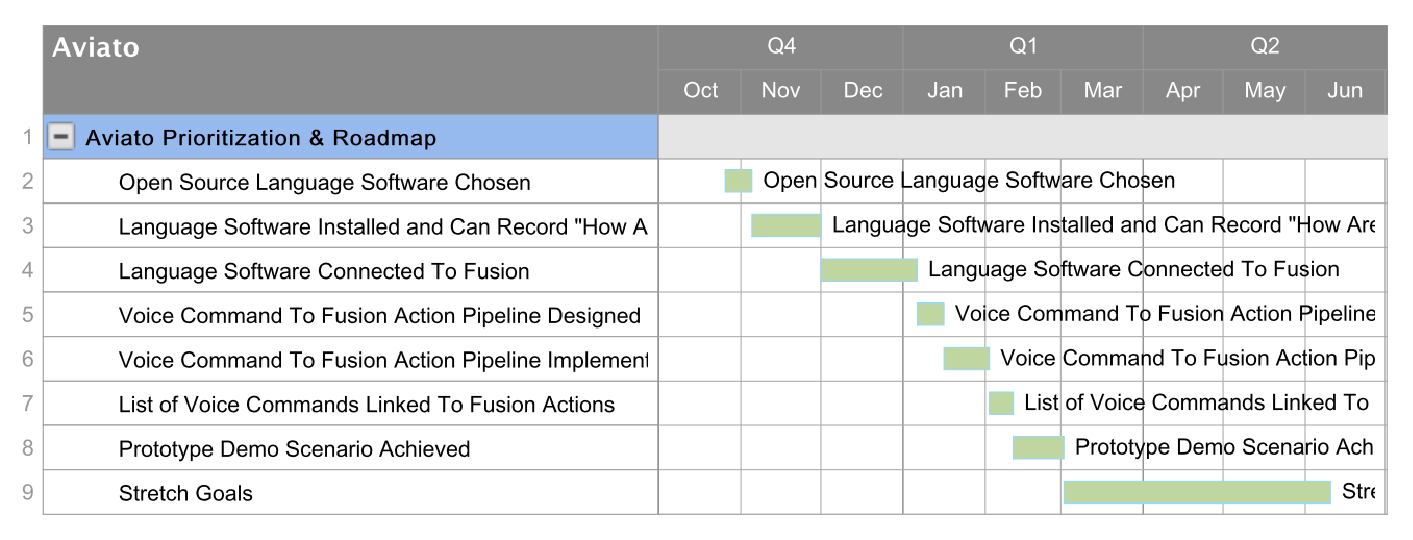
\includegraphics[width=1\textwidth]{ganttChart.eps}
			%Changed Gantt chart to be modifiable.
			\begin{ganttchart}[
				y unit title=0.4cm,
				y unit chart=0.5cm,
				vgrid,
				hgrid,
				title left shift=.05,
				title right shift=.05,
				title height=1,
				group right shift=0
				]{1}{24}
				\gantttitle{Months}{24} \\
				\gantttitle{January}{4}
				\gantttitle{February}{4}
				\gantttitle{March}{4}
				\gantttitle{April}{4}
				\gantttitle{May}{4}
				\gantttitle{June}{4} \\


				\ganttbar{MongoDB Creation}{1}{2} \\
				\ganttbar{Module Skeletons Creation}{1}{2} \\
				\ganttbar{Speech-to-Intent Working}{2}{3} \\
				\ganttbar{Text-to-Speech Working}{3}{3} \\
				\ganttbar{Fusion API Mapping}{2}{5} \\
				\ganttbar{Pipeline Connected}{4}{9} \\
				\ganttbar{Alpha Demo Creation}{9}{11} \\
				\ganttbar{Performance Testing}{9}{12} \\
				\ganttbar{Train NLP Modules}{13}{20} \\
				\ganttbar{Beta Demo Creation}{17}{24} \\
				\ganttbar{Smart Assistant Stretch Goal}{15}{23} \\
				\ganttbar{Engineering Expo}{24}{24}

			\end{ganttchart}
			\captionsetup{justification=centering}
			\caption{\botname Development Schedule}
			\label{fig:developmentSchedule1}
		\end{center}
	\end{figure}


	\subsection{Conclusion}
	This document has described \botname's development roadmap.
	This document explains how \botname's underlying system is decomposed into components and what each component is responsible for.
	Above is a Gantt chart that details the development schedule which the \botname developers will abide by.
	There is a change history table at the beginning of this document which will explain any modifications made to the design described in this document.















\section{Tech Review}

	\subsection{Natural Language Processor}
	\subsubsection{Overview}
	As a voice assistant, \botname will be required to receive and understand speech from a user.
	In order to do this, a natural language processor will be needed to translate either the user's speech, or a transcript of the user's speech, into a program-usable form.
	This section will review and compare existing natural language processors that could be used to do this.

	\subsubsection{Criteria}
	There are several important aspects to consider when deciding what \botname will use to parse the user's raw language.
	The primary consideration is cost.
	This project is a proof-of-concept and thus requires only a working prototype and may not be put into production.
	Ideally it should not cost any money create.
	Therefore, a free option that can accomplish everything that is required by \botname is ideal.
	Other things that are taken into account are the processor's accuracy, implementation difficulty, and comprehension flexibility.
	An ideal choice is accurate with its interpretations of intent, is easy to implement, maintain, and modify, and is capable of mapping multiple similar phrases to the same intent.

	\subsubsection{Options}
	\subsubsection{Wit.ai}
	Wit.ai is Facebook's free-to-use open-source project for natural language processing\cite{WitFAQ}.
	It is capable of deriving intent directly from audio of a user speaking and provides a graphical user interface for developers.
	Also supported are automatic intent triggers, comprehension flexibility, and entity roles.
	There is extensive documentation for Wit.ai, however, all official examples are given in the context of an app that is integrated with Facebook Messenger\cite{NLPComparisons}.
	\subsubsection{Dialogflow}
	Dialogflow, formerly Api.ai, is Google's solution for natural language processing.
	To use Dialogflow in a large-scale enterprise environment, one the pay-to-use Enterprise plan would need to be purchased\cite{DialogflowPricing}, thus this is considered an option that is not free.
	While not free to use, Dialogflow does offer a feature-rich language processing tool with a developer user interface.
	It supports automatic intent triggers and comprehension flexibility and comes with built-in functionality specifically for chat bots.
	It is capable of processing directly from speech audio and is even capable of automatically querying the user for missing information needed to accurately derive intent\cite{NLPComparisons}.
	\subsubsection{Alexa}
	Amazon has provided developers with free access to Alexa Skills Kit for implementing new functionality in Alexa-integrated apps and devices.
	The provided development kit offers speech-to-intent processing capabilities, but the accuracy and ability to learn new phrases are described as weak by some.
	While the kit offers language processing capabilities, it requires that all interactions and responses are handled manually in the business logic.
	Alexa's diagnostic tools are also limited\cite{NLPComparisons}.

	\subsubsection{Comparison}
	\begin{table}[H]
		\begin{center}
			\begin{tabular}{|c|c|c|c|c|c|}
				\hline
				& Processes Audio & Free & Automatic Interaction Handling & Comprehension Flexibility & Developer UI \\
				\hline
				Wit.ai & \greencheck & \greencheck & \greencheck &  \greencheck & \greencheck \\
				\hline
				Dialogflow & \greencheck & \redcheck & \greencheck & \greencheck & \greencheck \\
				\hline
				Alexa & \greencheck & \greencheck & \redcheck &  \redcheck &  \redcheck \\
				\hline
			\end{tabular}
			\caption{NLP Feature Comparison Chart}\label{tab:NLPFeatCompare}
		\end{center}
	\end{table}

	\noindent Wit.ai, Dialogflow, and Alexa all offer functionality that could be used to implement the natural language processing aspect of \botname.
	However, there are differences that separate them.
	Wit.ai and Dialogflow offer the best developer experience for ease of implementation and use.
	Both of these options have developer user interfaces, automatic interaction handling, and the ability to comprehend variations of the same phrases.
	The Alexa Skills Kit lacks all three of these features and thus would be more difficult to develop with.
	However, while Alexa may lack some usability features, it and Wit.ai are free to use while Dialogflow would require some level of spending.
	All three choices offer the ability to process audio directly which eliminates the need for \botname to transcribe a user's voice commands to text.

	\subsubsection{Conclusion}
	Wit.ai is the clear best choice for \botname's natural language processing component.
	It is the only one of the three presented options that both offers rich usability features and is free.
	For this reason, Wit.ai will be the natural language processor used by \botname.

	\subsection{User Action Prediction}
	\subsubsection{Overview}
	One aspect of the stretch goal for this project is adding the ability to predict the user's commands before they are given.
	To do this, \botname will need to incorporate some form of machine learning so that it can learn the use patterns of each individual user.
	This section will review and compare available options for achieving this functionality.
	\subsubsection{Criteria}
	An ideal tool for implementing \botname's user action prediction functionality should be easy to learn and use and robust in its learning methods.
	Ease of use is a particularly important feature as the time frame for implementing this functionality will likely be short and none of the developers working on this project have prior experience in machine learning.
	\subsubsection{Options}
	\subsubsection{Self-Implemented Process}
	There are many models that are used for predictive analysis and any of them could be implemented from scratch.
	This method would provide the ability to customize the smallest detail of the machine learning process to the project since the project developers would have to specify every aspect of the process.
	Implementing this option would require extra time for at least one developer to research implementation methods.
	\subsubsection{Scikit-learn}
	Scikit-learn is a robust machine learning library for Python that offers predefined processes for performing many learning techniques such as regression analysis, data clustering, and object classification\cite{ScikitLearnOrg}.
	The primary advantage of this option is that using it would minimize the amount of time spent researching by a developer since it comes with most of the necessary functionality.
	The one potential disadvantage of using scikit-learn is that the library does not support deep learning and thus that technique would not be available\cite{ScikitLearnDeepLearning}.
	\subsubsection{Tensorflow}
	Tensorflow is a library released by the Google Brain team that offers pre-built graph structures and methods to perform deep learning\cite{TensorflowOrg}.
	Using this option would offer the ability to implement the prediction model as a neural net which is considered a robust learning technique.
	The disadvantage of this library is that it restricts the learning methods to deep learning and requires more research to use effectively than scikit-learn.
	\subsubsection{Comparison}
	Self-implementing a prediction model from scratch would offer the most control over the process, however, it would be difficult and time-consuming to implement a process with learning capabilities equal to existing pre-built options.
	Scikit-learn offers the greatest ease of use of all the options and has more learning methods available than Tensorflow.
	Tensorflow's one advantage is that it offers the ability to do deep learning.
	\subsubsection{Conclusion}
	Scikit-learn fulfills the criteria best as it is the easiest to use without prior machine learning knowledge and offers a varied set of options that is only matched by self-implementing a predictive model which is itself unrealistic for the given time constraints.
	If in a late stage of the project it is realized that deep learning is needed for this component of the project, Tensorflow can be integrated and used in conjunction with scikit-learn.

	\subsection{Development Language}
	\subsubsection{Overview}
	The interactions between the various libraries and APIs being used in this project will need to be handled by some business logic implemented by the project developers.
	With that in mind, it is necessary to decide what programming language will be used.
	\subsubsection{Criteria}
	The chosen language should be supported by the various libraries and APIs being used in the project.
	It should also be fast enough that there are no noticeable performance issues, i.e. runtime delays, as a result from using it.
	Relative modifiability of code written in the language should be taken into account as well.
	\subsubsection{Options}
	\subsubsection{Python}
	Python is supported by the Fusion API as well as the chosen speech processor, Wit.ai, and the selected machine learning library, scikit-learn.
	It is a language that is fast for prototyping and has highly readable syntax which often times makes it easier to make changes to existing code.
	The disadvantage to using Python is that it is often noted as being far slower to run than other languages\cite{PyCppSpeedBenchmarks} and therefore is often replaced between the prototyping and production stages with a language that is faster.
	\subsubsection{C++}
	C++ is supported by the Fusion API, however it is not supported by the chosen speech processor, Wit.ai, nor the selected machine learning library, scikit-learn.
	Despite this, there are other speech processing and machine learning libraries that could be used with C++.
	The language is relatively low-level and requires developers to implement some functionality manually that already exists in other languages such as memory management.
	An advantage that stems from this is that C++ is a relatively fast language\cite{PyCppSpeedBenchmarks}.
	\subsubsection{Other}
	No other language is supported by the Fusion API.
	However, there are advantages to other languages with respect to other parts of the project.
	For example, the R programming language is one of the most popular for data analytics and thus machine learning\cite{MLLang} while implementing speech recognition with Node.js would allow easy future integration of other Google libraries for additional functionality.

	\subsubsection{Comparison}
	No languages other than Python and C++ are supported by the Fusion API\cite{AutodeskCreateScript}, a necessary part of the project, and therefore no others will be considered.
	Python is fast to develop in, highly modifiable, and feature-rich while using C++ results in reduced development speed, less modifiability, and fewer features to use in development.
	However, the use of C++ would make the application much faster than if it were implemented using Python.

	\subsubsection{Conclusion}
	This project will be implemented using Python.
	The duties that will be handled in the business logic are small enough that the slower speed of Python should not result in any performance losses that are noticeable to the user.
	The access to the features that are supported with Python and the ability to write modifiable code quickly are aspects of the language that will be advantageous to the implementation of this project.



	\subsection{Log File Storage}
	Kora will be storing log files that describe user interactions with her.
	Storing user-Kora interactions has three main uses: debugging, feature additions, and machine learning possibilities.
	It will be much easier to debug technical problems when a play-by-play of actions leading up to the crash is given to the developer.
	Storing what commands users are asking Kora to execute allows for easy feature additions without the need to survey users for what commands Kora is lacking.
	For instance, if a number of users are asking "Kora, convert the file to STL format" and Kora doesn't have that capability yet the logs will show that.
	This allows developers to easily understand what users would like Kora to do.
	Storing the commands users are asking Kora to execute as well as answers to Kora's interview questions allows for machine learning by allowing Kora to learn ways to better assist the user based off of previous patterns.

	\subsubsection{Criteria}
	Kora needs the ability to store log files quickly, as she will be annotating every interaction she is a part of.
	She needs the ability to easily access the contents of the files, but not necessarily with 100\% transaction safety.
	The log file structure must be easily mutable because as Kora matures she will gain more skills, meaning she will have more to record from her interactions.
	The team may also come across new fields that she should begin recording.
	The structure must also be easily scaled, because as Kora attracts more users the amount of log files being stored will go up a great amount.


	\subsubsection{MySQL: Relational Database}
	A relational database is a rigid, structured way of storing data.
	The relationship between tables and field types is called a schema.
	In a relational database, the schema must be clearly defined before any information can be added.
	For a relational database to be effective, the data being stored has to be structured in a very organized way with all fields of the table filled, no more no less. 
	Because relational databases are well structured they support the JOIN clause which allows developers to retrieve related data stored across multiple tables with a single command.
	MySQL database tables must explicitly mention what other tables they rely on.
	Due to this, it's impossible for users to add, edit or remove records which could result in invalid data or orphan records \cite{SQLvsNoSQLsitepoint}.

	\textbf{Pros:}
	\begin{itemize}
		\item{
			Referential data integrity}
		\item{
			Supports complex queries}
		\item{
			Very organized structure}
		\item{
			High level of transaction safety}
	\end{itemize}
	\textbf{Cons:}
	\begin{itemize}
		\item{
			If the schema needs to change, then the entire database needs to be edited \cite{SQLvsNoSQLupwork} }
		\item{
			Challenging to scale}

	\end{itemize}

	\subsubsection{MongoDB: Non-Relational Database}
	MongoDB is a NoSQL non-relational database.
	Instead of tables, NoSQL databases are document-oriented.
	Non-relational databases are more like file folders with key-value pairs, which assemble related information regardless of type. 
	This means there is no enforced structure to the data, meaning all inserts don't have to be structured identically with the same keys.
	This way, non-structured data can be stored in a single document that can be easily found but isn't necessarily categorized into fields like a relational database is. 
	MongoDB by default prefers high insert rate over transaction safety.
	Generally database scaling in hard.
	However, if one needs to partition and shard the database, MongoDB has a built in easy solution for that \cite{SQLvsNoSQLupwork}.

	\textbf{Pros:}
	\begin{itemize}
		\item{
			NoSQL databases offer ease of access to data.
			MongoDB has APIs which allow developers to execute queries without having to learn SQL or understand the underlying architecture of their database system.}
		\item{
			Can store large volumes of data that have little to no structure} 
		\item{
			Designed to be scaled across multiple data centers and servers}
		\item{
			Rapid development. NoSQL data doesn’t need to be prepped ahead of time \cite{SQLvsNoSQLupwork}}
	\end{itemize}

	\textbf{Cons:}
	\begin{itemize}
		\item{
			Non-relational databases like MongoDB don't support the JOIN clause which allows developers to retrieve related data stored across multiple tables with a single command}
		\item{
			Generally, storing data in bulk requires extra processing effort and more storage than highly organized relational data \cite{SQLvsNoSQLupwork}}
	\end{itemize}


	\subsubsection{Local File System}
	Storing log files locally would consist of a log folder which holds all the log files.
	The log file would be made up of delimited rows where each row would contain data pertaining to a user-Kora interaction.
	A new log file would be created when a certain circumstance is met, such as the beginning of a new day or X amount of entries.

	\textbf{Pros:}
	\begin{itemize}
		\item{
			No database overhead}
		\item{
			Direct access to logs}
		\item{
			No structure or language specific constraints}
	\end{itemize}
	\textbf{Cons:}
	\begin{itemize}
		\item{
			Challenging to query}
		\item{
			Hard to scale}
		\item{
			Possibly not reader friendly}
	\end{itemize}
	\subsubsection{Conclusion}
	Storing log files locally in a log folder isn't practicable to meet the goals log files are trying to achieve.
	There isn't an easy way to query them for data and in the long term the file system would be covered in files since Kora needs to archive them for learning purposes.
	The choice now comes down to MongoDB and MySQL.
	MySQL is very structured, which allows for complex data queries.
	However, the majority of Kora's work will be insertions not reads.

	MongoDB is chosen over MySQL for the following reasons.
	\begin{enumerate}
		\item{
			The data associated with user-Kora interactions are changing.
			As Kora evolves more characteristics of the interaction will be stored.
			MongoDB doesn't have a structured schema, so additions and subtractions of data fields is simple.
			Whereas MySQL requires all predefined fields to be filled in, and additions and subtractions of fields requires an entire database update}
		\item{
			Non-relational databases are designed to be scaled.
			As Kora evolves the amount of log files will only continue to increase, and they must be archived for machine learning reasons described above.
			MySQL on the other hand, doesn't scale well \cite{SQLvsNoSQLsitepoint}.}
		\item{
			MongoDB by default prefers high insert rate over transaction safety \cite{SQLvsNoSQLupwork}.
			As Kora attracts more users the amount of writes to the database will increase tremendously.
			Transaction safety isn't a factor that needs to be taken into account, as data here and there could be missing or corrupt and the overall goals of the log files could still be accomplished.}
	\end{enumerate}

	It's possible to choose MongoDB and switch to MySQL later.
	If the team discovers a MySQL database would better suit the project it's possible to migrate the data to one.




	\subsection{Mapping Text to a Fusion Command}
	There are two components to executing a voice command.
	The first is understanding.
	Kora must be able to listen and transcribe what the user is requesting.
	The second is the actual execution of the command.
	Kora needs to know how to execute the request.
	For example, if Kora hears and transcribes "rotate the design 90 degrees", she needs to know to call the Fusion API's \textit{rotation} endpoint.

	\subsubsection{Criteria}
	The solution should be robust enough that if Kora is capable of executing the Fusion command, she maps the text to it accordingly, there is no ambiguity.
	The addition of new mappings should be an easy process.


	\subsubsection{Utterance Templates}
	Utterance templates could be created to do this.
	In this context, an utterance is a phrase that is spoken which signals a specific command.
	A few example utterances for saving a design would be: "Save design as myDesign1", "Save design", and "Please save the current design as myDesign1."
	All of these phrases should correspond to the Fusion API \textit{save} endpoint.
	An utterance can have variables, called slots, throughout the phrase that can accept any slot predefined value or type.
	For example, "save design as \{name\}" where \{name\} is a slot value that is set to accept any alphanumeric string.
	A data structure would be constructed where the elements of the structure are the Fusion commands, and they are signaled if any of their utterances are met.

	\textbf{Pros:}
	\begin{itemize}
		\item{
			Developer friendly to read and understand}
		\item{
			Structured (little uncertainty in what the outcome will be)}
		\item{
			Easy to add new commands and phrases}
	\end{itemize}

	\textbf{Cons:}
	\begin{itemize}
		\item{
			Have to create template architecture from scratch}
		\item{
			Time consuming to create utterances}
		\item{
			The reliability of the mapping is dependent upon having a wide variety of utterances.
			This may make it challenging to verify that the most commonly used phrases to execute a command are stored as utterances.}
	\end{itemize}



	\subsubsection{Keywords}
	The idea behind the keywords solution is to execute Fusion commands based off of keywords in the transcribed command.
	This simple solution would create a key-value pair table where the key is a keyword that can show up in a command and the value is the Fusion API call to make.
	Kora would scan through the spoken command to see if there is a keyword that is stored in the command table.
	If there is, then Kora would execute the mapped command.
	Let's say \textit{save} is a keyword.
	If the user said "save the design", then Kora would scan through the sentence and notice the keyword \textit{save}.
	Kora would realize that \textit{save} is in the command table and execute the corresponding Fusion API call to save the design.

	\textbf{Pros:}
	\begin{itemize}
		\item{
			Simpler to implement}
	\end{itemize}

	\textbf{Cons:}
	\begin{itemize}
		\item{
			Ambiguity in what command Kora should execute if there are multiple keywords in the transcribed command}
		\item{
			No quantities or details of a command. Rotate, but by how much and which way? Save design, but by what name? }
		\item{
			Far less durable and scalable than other options due to the ambiguity}
	\end{itemize}


	\subsubsection{Amazon's Alexa Skills Kit}
	The Amazon's Alexa Skills Kit solution is entirely dependent upon if Alexa is used as Kora's voice synthesizer.
	Amazon's Alexa is a full-fledged voice command software that supports voice-to-text and text-to-voice software.
	After Alexa synthesizes the voice command she checks her skills collection and sees if the request is something she can execute.
	Her skills are called Alexa skills and they are roughly implemented in the way same way that the templates I described above are.
	A command is executed if one of the utterances for it is met.
	To teach Alexa a new skill is as simple as following the process outlined in Alexa's documentation.
	The storage and implementation of the skill into Alexa's skill collection is taken care of behind the scenes by Alexa \cite{alexaSkills}.

	\textbf{Pros:}
	\begin{itemize}
		\item{
			Architecture is already produced}
		\item{
			Easy to add new commands and phrases}
		\item{
			Back-end complexities such as adding the skill to the skill collection is taken care of behind the scenes by Alexa}
		\item{
			Reliable}
	\end{itemize}

	\textbf{Cons:}
	\begin{itemize}
		\item{
			Potentially tedious to create utterances}
		\item{
			Challenging to verify that the most commonly used phrases to execute a command are stored as utterances}
	\end{itemize}


	\subsubsection{Conclusion}
	The keywords solution isn't practicable due to the ambiguity that can and will take place in figuring out which command to execute.
	There is no durable solution to extracting quantities and specifics of a request using the keyword solution.
	The templates solution is very similar to how the Alexa Skills Kit adds new skills.

	The Alexa skills solutions is the best choice due to the following reasons.
	\begin{enumerate}
		\item{
			The team wouldn't have to develop the skills architecture because it's already setup and thoroughly tested by Amazon.}
		\item{
			Alexa has an easy to use API for adding new skills.
			This means that all of the complexities that come along with instructing the software to use the new skill is taken on by Alexa behind the scenes.}
		\item{
			Alexa has proven her reliability by the public acceptance.}
		\item{
			There is a vast amount of documentation and helpful resources online.}
	\end{enumerate}

	If Alexa is not the chosen voice synthesizer then the next best choice would be the templates solution as it is more durable and scalable than the keywords solution.


	\subsection{Awakening Kora}
	Voice controlled devices aren't always listening for commands to execute.
	A user needs to signal the software if they would like to execute a command.
	Industry examples of this are Google's "Okay Google," and Microsoft's "Hey Cortana."

	\subsubsection{Criteria}
	Awakening Kora should take no longer than two seconds.
	The process should stick to one step.
	Awakening Kora should not be a tedious process.

	\subsubsection{Wake Word}
	Wake words must meet two conditions: they shouldn't be triggered by accident and they should be unique across all languages.
	With that being said, the name Kora is uncommon and unique across all languages.
	Amazon's Alexa's default wake word is simply "Alexa", and Apple's Siri's wake word is simply "Siri."
	Amazon and Apple are big companies that most likely put a great deal of resources into figuring out a user friendly wake phrase.
	So, I believe having Kora's wake word simply being "Kora" is a valid solution.
	Examples of this are "Kora, rotate design 90 degrees to the left" and "Kora, save design as myDesign1"

	\textbf{Pros:}
	\begin{itemize}
		\item{
			Hands free}
		\item{
			It's used by big companies, meaning it has public acceptance}
		\item{
			It's one step}
	\end{itemize}

	\textbf{Cons:}
	\begin{itemize}
		\item{
			Potentially not ideal if Kora commands are asked frequently, as saying Kora repeatedly is tedious}
	\end{itemize}


	\subsubsection{Button Press}
	Since the user is interacting with Kora within Fusion, another viable solution would be to have a Kora button in the toolbar.
	When the Kora button is pressed Kora awakens and begins listening for a command from the user.
	Examples of this are \textit{press Kora button} "Rotate design 90 degrees" and  \textit{press Kora button} "Save design as myDesign1"

	\textbf{Pros:}
	\begin{itemize}
		\item{
			No chance of accidentally executing a command}
		\item{
			Takes less than two seconds}
	\end{itemize}

	\textbf{Cons:}
	\begin{itemize}
		\item{
			Inefficient because the mouse has to leave the design or current work space}
		\item{
			Tedious}
	\end{itemize}


	\subsubsection{Teammate Mode}
	Teammate mode is similar to the button press option, except the Kora button doesn't signal Kora that a command is coming.
	Instead, it turns Kora on and puts her in teammate mode where she is constantly listening for commands until she is taken out of teammate mode.
	When Kora is not in teammate mode commands don't execute because Kora isn't listening.
	In teammate mode there is no need to say "Kora" at the beginning of the command, because she is already listening.
	Examples of this are \textit{press Kora teammate mode button}\dots user working \dots "rotate design 90 degrees to the left" \dots user continues working \dots"save design as myDesign1."

	\textbf{Pros:}
	\begin{itemize}
		\item{
			No need to repetitively say a wake work}
		\item{
			No need to repetitively press a button}
	\end{itemize}

	\textbf{Cons:}
	\begin{itemize}
		\item{
			User must be in a quite area so background chatter doesn't execute a command}
		\item{
			Kora executing commands it hears from the background will annoy users}
	\end{itemize}


	\subsubsection{Conclusion}
	Due to the Kora team not having access to the Fusion source code, the button press and teammate mode options may not be possible as they would require Fusion to communicate with the external voice control software, which may not be possible through the Fusion API.
	For that reason, the wake word "Kora" will be used before each command to awake Kora.
	This is a good solution because it is hands free, takes less than two seconds to say, is one step, and most users are already used to interacting with voice control software via a wake word.















\clearpage

\section{Weekly Blog Posts}
	\begin{center}
		\begin{longtabu} to \textwidth {|X[2,l]|X[8,l]|X[8,l]|}
			\hline
			& \textbf{\Large{Jeremy}} & \textbf{\Large{Austin}}  \\ \hline
			&	\textbf{\large{Fall Term 2017}}  &\\ \hline
			\textbf{Week} & \textbf{Summary}  & \textbf{Summary }\\ \hline

			Week 1
			&
			{
				This week I updated my resume and professional biography for class. I also emailed Patti regarding the capstone project. The project involves Natural Language Processing (NLP) , so I found a YouTube video series on NLP taught by two Stanford professors and watched a handful of those. I also researched some NLP methods that I learned from those videos.
			}

			&
			{
				This week involved a small collection of tasks to prepare for the class as a whole.
				I wrote and posted the Professional Biography and reviewed my resume for the in-class editing activity.
				I also submitted my project preferences for project selection.
			}
			\\ \hline

			Week 2
			&
			{
				The team reached out to Patti and set up an introductory meeting from 8:00 - 8:30am on Friday October 6th. The meeting went good. We got an overview of what Autodesk does, as well as Patti's role. We touched on the project and what she's hoping to get out of it, but scheduled an hour long follow up meeting for Monday October 9th to dive deeper into the project.
			}

			&
			{
				This week I was assigned to my project and group.
				I met with my group mates and discussed the overarching idea for the project in a meeting with our client.
				We didn't get many details for our project out of our meeting so we have scheduled another one next Monday to discuss project specifics.
				We will have a better idea of exactly what we will be doing for our project after this meeting.
			}
			\\ \hline

			Week 3
			&
			{
				We met with Patti for about an hour Monday afternoon and got a better understanding of the project. The meeting notes can be found in 3.1. She mentioned that we won't be getting Fusion source code, we will have to use the Fusion APIs instead. This will be challenging, because we will have to figure out a way to work through the API to integrate the voice control libraries.

				I found an open source library called Mycroft that seems like the whole package: Voice-to-text, text-to-voice, sentence sentiment, and more. I haven't looked at it too deeply yet, but just from what I've seen so far I think there is a major obstacle to overcome If we want to use it. Mycroft is only supported on Raspberry Pis, android, and Linux because it is aimed towards embedded device. So, to get this running on Mac OS or Windows may not be possible. We'll see.
			}

 			&
			{
				This week we had another meeting with our client to discuss some of the details of our project and clarify exactly what she wants.
				We also drafted our problem statements and received in-class feedback.
				Looking forward we will aim to formulate specific project requirements and research tools that will help us meet these requirements.
			}
			\\ \hline

			Week 4
			&
			{
				\begin{itemize}
					\item Met with Juneki and discussed our GitHub repo structure. We need to add a Docs folder.
					\item Met with Patti on Thursday afternoon and went through the problem statement together
					\item We agreed on Phase 1 (our project) vs. Phase 2 (stretch goals) and accomplishments within each
					\item We created a scenario to demonstrate at Expo. This is our project goal.
				\end{itemize}
			}

			&
			{
				This week we reorganized our GitHub directory structure as per the instructions given to us by our TA in our weekly meeting, finished and submitted the final draft of the problem statement, and further discussed and clarified the goals of our project with our client.
				Next week we will start thinking more about smaller details of our project as we begin the requirements document.
			}
			\\ \hline

			Week 5
			&
			{
				\begin{itemize}
					\item This week we worked on the Requirements rough draft
					\item Met with Junki on Tuesday and discussed possible open source projects we could use
					\item Thursday meeting with Patti was canceled - she was traveling
				\end{itemize}
			}

			&
			{
				This week was dedicated specifically to writing the first draft of the requirements document.
				Patti cancelled the normal Thursday meeting since she was travelling for work.
				We had no problems creating this first draft.
				Next week we will look to finalize and submit the project requirements.
			}
			\\ \hline

			Week 6
			&
			{
				\begin{itemize}
					\item Met with Junki on Tuesday and discussed whether there was a research component to our project -- we agreed there was in our stretch goals
					\item Went to the research class on Thursday (see notes in 6.4)
					\item Met with Patti Thursday night and went through the requirements document. She liked it, and added a few things to think about
					Turned requirements document in.
				\end{itemize}
			}

			&
			{
				This week we finalized and submitted the project requirements after reviewing them with our client.
				We also attended the research lecture to learn about how to approach the research-oriented aspects of our project.
				We did not encounter any problems this week.
				Next week we will discuss how we intend to break up the project into different pieces for the technology review and may begin drafting our individual technology reviews.
			}
			\\ \hline

			Week 7
			&
			{
					\begin{itemize}
						\item The three of us had a meeting on Wednesday and discussed the nine parts of the project
						\item Met with Patti on Thursday and ran the nine parts by her. She approved
						\item She also mentioned that using Amazon's Alexa is a valid choice. She just wants to make sure we won't have to pay anything
						\item Divided the nine components into three each. I am in charge of…
						 \begin{itemize}
						 	\item Log File Storage
						 	\item Lexicon For Mapping Text to Fusion Command
						 	\item Interaction Model (wake words)
						 \end{itemize}
					\end{itemize}
			}

			&
			{
				This week was dedicated entirely to breaking the project into components for the tech review.
				This was difficult as there are really only a few core technologies that need to be linked together to implement our project.
				Patti, the client, said that she believed that we should add a discussion of methods for signaling to the assistant that it is being given a voice command and some others agreed.
				However, I'm not sure that this is actually an appropriate discussion for the technology review assignment.
				Next week We will complete and iterate upon our individual first drafts of the technology review assignment.
			}
			\\ \hline

			Week 8
			&
			{
				This week I completed the tech review. I researched the best data structure for storing log files, how to map text output by the voice synthesizer to a Fusion command, and how to awake Kora in an efficient user friendly fashion.
				Our weekly Thursday meeting with Patti got canceled because she was traveling.
			}

			&
			{
				This week I revised my tech review document to incorporate changes suggested during the in-class peer review.
				I sent the revised document to Patti for feedback.
				Next week we will start our design document.
				No problems were encountered this week.
			}
			\\ \hline

			Week 9
			&
			{
				I did absolutely nothing this week. There was school Monday, Tuesday, and Wednesday with Thursday and Friday off for Thanksgiving break. Next week I'll be working on and completing the Design Document and the Progress Report.
			}

			&
			{
				No progress was made this week as it is Thanksgiving week.
				As such, there were no problems.
				Next week our group will do the design document.
			}
			\\ \hline

			Week 10
			&
			{
				\begin{itemize}
					\item We finished the design document and the progress report.
					\item The meeting with Patti was canceled because she was traveling, however James, Austin, and I had a meeting and discussed how we were going to break down the design document and what parts went into it.
					\item Austin and I also had a long session mapping out Kora's design on a whiteboard. James wasn't there, but we met up with him after and showed him pictures of the design on the whiteboard. To see these pictures, check the General $\rightarrow$  Design Document page
				\end{itemize}
			}

			&
			{
				This week was dedicated entirely to the planning and completion of the first iteration of the design doc which was submitted on Friday.
				Thursday's usual meeting with Patti was cancelled due to her being unavailable.
				Next week will be finals/winter break and so we will start upon the second iteration of the design document.
				Our team's goal is to come back from winter break with every aspect of the project satisfactorily specified in the design document so that implementing the project will be easy and clean.
				This should keep the code structure from devolving into anything too messy and gives an ultimate reference for any potential implementation questions in the context of design.
				There were no problems this week.
			}
			\\ \hline








			% WINTER TERM
			&	\textbf{\large{Winter Term 2018}}  &\\ \hline

			Week 1
			&
			{
				\begin{itemize}
					\item Set up the new meeting time with Junki
					\item Set up a meeting with Patti and the new project clients
					\item Researched HTTP APIs for MongoDB
				\end{itemize}
			}

			&
			{
				This week we tackled the issue of how to allow Kora to use non-standard Python libraries since the code runs in an isolated environment with access only to standard python libraries.
				We bundled the source of the libraries that we want to use into the directory containing Kora and use all relative imports to get around this as it is the method suggested by the Fusion API developers.
				Looking forward we will begin to try to get the save and rotate commands to work in the editor through Kora.
			}
			\\ \hline

			Week 2
			&
			{
				\begin{itemize}
					\item Met with Anand, Rob, Patti, and Austin. James was sick so he couldn't make the call. Anand and Rob are very excited to be a part of the project.
					\item I set the github repo up inside of Fusion so Kora runs as a script in the Add-Ins section.
					\item I finished setting up the database locally
				\end{itemize}
			}

			&
			{
				This week we met the individuals at Autodesk who will be taking over our project in February when Patti officially leaves the company.
				We also got rotation to partially work in the editor.
				Given a command to rotate by a certain amount in a certain direction, Kora will rotate the object in the editor in the correct direction, but not by the correct amount.
				Next week will be focused on get the magnitude of rotation right and implementing the save command.
			}
			\\ \hline

			Week 3
			&
			{
				\begin{itemize}
					\item Helped James set up the repo in Fusion
					\item Met with Junki to discuss current progress and alpha demo deadlines
					\item Met with Austin and discussed transitioning Kora from a script to an Add-In
					\item Got PyAudio working and a successful API call
				\end{itemize}
			}

			&
			{
				This week we discovered that the Fusion 360 editor runs Add Ins on the same thread as the editor itself and therefore does not inherently support running Add Ins in the background.
				We managed to get Kora to run in the background anyway using Python's threading module and firing events that briefly return control of the main thread back to the Kora Add In for executing code that can only be executed in the main thread.
				There are several features not yet taken on the Kanban board including devising a testing framework for Kora so that is likely what I will work on next week.
			}
			\\ \hline

			Week 4
			&
			{
				\begin{itemize}
					\item Met with Junki and discussed the Poster and Midterm progress report coming up
					\item Set Kora up as an Add-In. At first we ran into a problem with the tkinter library causing Fusion on Mac to slowly crash. We resorted back to Fusion's built in message box to fix the problem (but it was a hassle to see where it was failing)
					\item Made progress on integrating database calls into Kora to log User-Kora interactions. It took awhile to lay the ground work because Fusion only plays nice with relative imports. So, I had to go through the entire mongoengine library and change its imports to relative imports.
				\end{itemize}
			}

			&
			{
				This week was largely dedicated to classes other than capstone.
				However, I did manage to solve the issue of having to manually train WIT's NLP model one example at a time by using selenium to automatically generate and validate training examples on the Wit.ai website.
				Next week I will look at getting the UI elements of Kora implemented.
			}
			\\ \hline

			Week 5
			&
			{
				\begin{itemize}
					\item Met with Anand and Jennifer and talked about progress, upcoming progress report, and going up to Autodesk after Expo to give a talk and demo.
					\item Finished MongoDB set up and code to log every User-Interaction. Instructions below.
					\item James unfortunately dropped the class so it is just Austin and I now.
					\item MongoDB is set up and correctly saves a User-Kora interaction
				\end{itemize}
			}

			&
			{
				This week along with our weekly meeting we developed elevator pitches for our project in class and created the first draft of our poster for expo.
				No new problems arose.
				Next week we will complete the Winter midterm progress report.
			}
			\\ \hline

			Week 6
			&
			{
				\begin{itemize}
					\item Met with Jennifer and talked about the preogress report coming up
					\item Met with Junki and talked about the progress report and poster.
					\item Created the progress report video and turned it in
					\item Created a general config file that has WIT access token and debug mode. If debug is on then know user-interactions get stored in the database.
					\item Created the save and save as command and trained WIT to recognize these commands
				\end{itemize}
			}

			&
			{
				This week was dedicated to reflecting on the first half of the development process for Kora and completing the progress report.
				We encountered no particular difficulties in doing this.
				Next week we will either begin looking into alternatives to Wit for performing Kora's NLP responsibilities or will begin implementing Kora's associated GUI components.
			}
			\\ \hline

			Week 7
			&
			{
				\begin{itemize}
					\item Placed an issue on WIT.ai GitHub account about the latency issue we are having. Apparently the latency used to be ~.5seconds and now that they are attempting to scale their software they have been running into latency issues. We are waiting to here back from them
					\item Jennifer mentioned not to worry about the latency at the moment and to work on our other requirements.
					Moving forward we will be implementing a UI and making Kora not crash on silence.
				\end{itemize}
			}

			&
			{
				We started this week by looking into alternatives to Wit for Kora's natural language processing functionalities.
				Upon determining that implementing an alternative may be a larger undertaking than previously expected, and with the advice of our client, we decided to leave the NLP latency issues for now and focus on  completing the other remaining project requirements.
				At the end of the week, we started looking at implementing the GUI components of Kora and will continue to work on that into next week.
			}
			\\ \hline

			Week 8
			&
			{
					Added code so that Kora doesn’t fire an event unless WIT (our NLP) returns something useful. The way it was previously set up is even if I said "I like chocolate cake and ice cream" Kora would still fire an event to execute the command in Fusion. This also caused an issue later on in the pipeline if WIT returned nonsense since it got white-noise. Now, when WIT responds we tell Kora to disregard the WIT response and keep listening if the response doesn’t have an "Intent" key, or if it does, but the confidence in the "Intent" value is less than the threshold (which is set at 79\%)
			}

			&
			{
				This was the week that we started implementing Kora's UI for status messaging and onboarding with PyQt, a Python GUI framework.
				By the end of the week, we discovered that none of the available Python GUI frameworks are going to work for what we want to do since they don't work properly in separate threads.
				We will go back to looking for options within the Fusion API for implementing Kora's UI next week.
			}
			\\ \hline

			Week 9
			&
			{
				Successfully implemented the 'Extrude' command for Kora. The only "issue" is that it doesn't look user friendly at the moment due to not being able to use a command dialog because using a command dialog doesn't allow us to return a \textit{executionStatusCode}.
			}

			&
			{
				This week we transitioned to using the Palette object provided by the Fusion API to implement Kora's UI for status messaging and onboarding.
				We ran into problems when trying to communicate between the AddIn and the palette and discovered that it was a bug in the API.
				Jennifer and Anand are going to talk to the API team to try to resolve this.
				Next week we will continue the implementation of the UI.
			}
			\\ \hline

			Week 10
			&
			{
				\begin{itemize}
					\item Looked at WakeWord software
					\item Popular software called Snowboy, but even the demo Seg-Faults on Mac. Spent about 3 hours trying to figure it out/tweak things and still didn’t get it to work.
					May switch gears and start looking into NLP projects that have the wake word included in them, since we may have to pivot away from Wit.ai to reduce the latency anyway
				\end{itemize}
			}
			&
			{
				This week we worked around the issues we were having in implementing Kora's feedback messaging with Fusion's Palette object by using a different HTML template for each of the messages and switching to a new template when appropriate.
				Next week we will focus on putting together the Winter Progress Report.
			}
			\\ \hline








			% SPRING TERM
			&	\textbf{\large{Spring  Term 2018}}  & \\ \hline

			Week 1
			&
			{
				\begin{itemize}
					\item Met with Jennifer and Anand and talked about our progress report and what they thought about it
					\item No meetings with Junki
					\item Started looking into Hot Word detection software: Snowboy and PocketSphinx
				\end{itemize}
			}

			&
			{
				No progress was made this week.
				Next week we will look into implementing a hot word for activating Kora.
			}
			\\ \hline

			Week 2
			&
			{
				\begin{itemize}
					\item Meeting with Junki cancelled
					\item Spent many hours trying to get Snowboy working.
					\begin{itemize}
						\item I'm assuming there is a problem with Snowboy on Mac, because even their demo that you can download off of their website Seg Faults
						\item I tried Pip installing it.     Didn't work, Seg Faulted
						\item I tried git cloning it, building it, running it.     Didn't work, Python crashed and Mac spit out a long log file
						\item Austin will try getting it on his Windows computer
					\end{itemize}
				\end{itemize}
			}

			&
			{
				We looked into but were unable to implement the use of an activation phrase for Kora.
				Next week we will continue to look into this.
			}
			\\ \hline

			Week 3
			&
			{
				\begin{itemize}
					\item Experimented with Pocket Sphinx. Specifically using it for Hot Word detection
					\item So far haven't been able to get it to work. There's no specific Mac version, just Linux. So that's probably why
					\item Researching other Hot Word detection software, and thinking of ways to do it on our own.
				\end{itemize}
			}

			&
			{
				We looked into but were unable to implement the use of an activation phrase for Kora.
				We also completed the WIRED article assignment.
				Next week will be spent making preparations to present the project to Autodesk employees.
			}
			\\ \hline

			Week 4
			&
			{
				\begin{itemize}
					\item Going Up to Autodesk on Friday to present our project to whoever attends. Anand said he's trying to get as many executives to show up as possible
					\item No progress as far as coding Kora goes
					\item Worked on putting together the presentation for Friday
					\item Presentation went good. About 40 people in person and 5 called in from SF via Skype.
				\end{itemize}
			}

			&
			{
				This week we prepared for and gave a presentation on our project to Autodesk employee's at their Portland office.
				Next week we will complete the midterm progress report.
			}
			\\ \hline

			Week 5
			&
			{
				\begin{itemize}
					\item Made corrections to the poster that Kirsten suggested
					\item Submitted the poster
					\item Worked on the midterm progress report.
				\end{itemize}
			}

			&
			{
				This week we completed the midterm progress report.
				We will make final preparations for expo next week.
			}
			\\ \hline

			Week 6
			&
			{
				\begin{itemize}
					\item Edited the requirements document. Specifically took the onboarding and wake word and loosened the latency metric.
					\item The onboarding wasn't doable throw the API and Fusion doesn't allow external GUIs to be used
					\item The Wake Word believe it or not was really hard to do. None of the open source libraries worked (the demos didn't even run), so we looked into do it ourselves. This is tricky because you have to always be recording and Saving that recording, because if you hear and interpret "Kora" then you have to work backwards in your recording and figure out what the audio was after "Kora" was said, and then send that up to WIT.
					\item The latency metric was loosened to "at most three seconds longer then it would take to do manually" (which is about where we are at) since WIT.ai was the NLP we went with and the latency was from their end.
					\item Got the edits approved by Anand and Jennifer
				\end{itemize}
			}

			&
			{
				We finished preparations for expo then went to expo.
			}
			\\ \hline

			Week 7
			&
			{
				\begin{itemize}
					\item We had expo this week
					\item We put together three separate videos to show at expo and included subtitles so the visitors can see what is being said.
					\begin{enumerate}
						\item Demo of all of our commands
						\item Demo showing the database contents we are storing
						\item Demo of training WIT.ai with Selenium
					\end{enumerate}
				\item Canceled our meeting with Anand and Jennifer because they didn't have anything to discuss and wanted to let us focus on expo.
				\end{itemize}
			}

			&
			{
				Working on final report and presentation.
			}
			\\ \hline

			Week 8
			&
			{
				\begin{itemize}
					\item Worked on Final Report
					\item Submitted peer evaluation
				\end{itemize}
			}

			&
			{
				Working on final report and presentation.
			}
			\\ \hline

			Week 9
			&
			{
				\begin{itemize}
					\item Worked on Final Report
					\item Worked on Final Presentation
					\item Worked on Documentation, readme, etc. for project to send to clients
				\end{itemize}
			}

			&
			{
				Working on final report and presentation.
			}
			\\ \hline

			Week 10
			&
			{
				Worked on Final Report
			}

			&
			{
				Completed and submitted final report and presentation.
			}
			\\ \hline

		\end{longtabu}
	\end{center}












\section{Final Poster}
	\begin{figure}[H]
		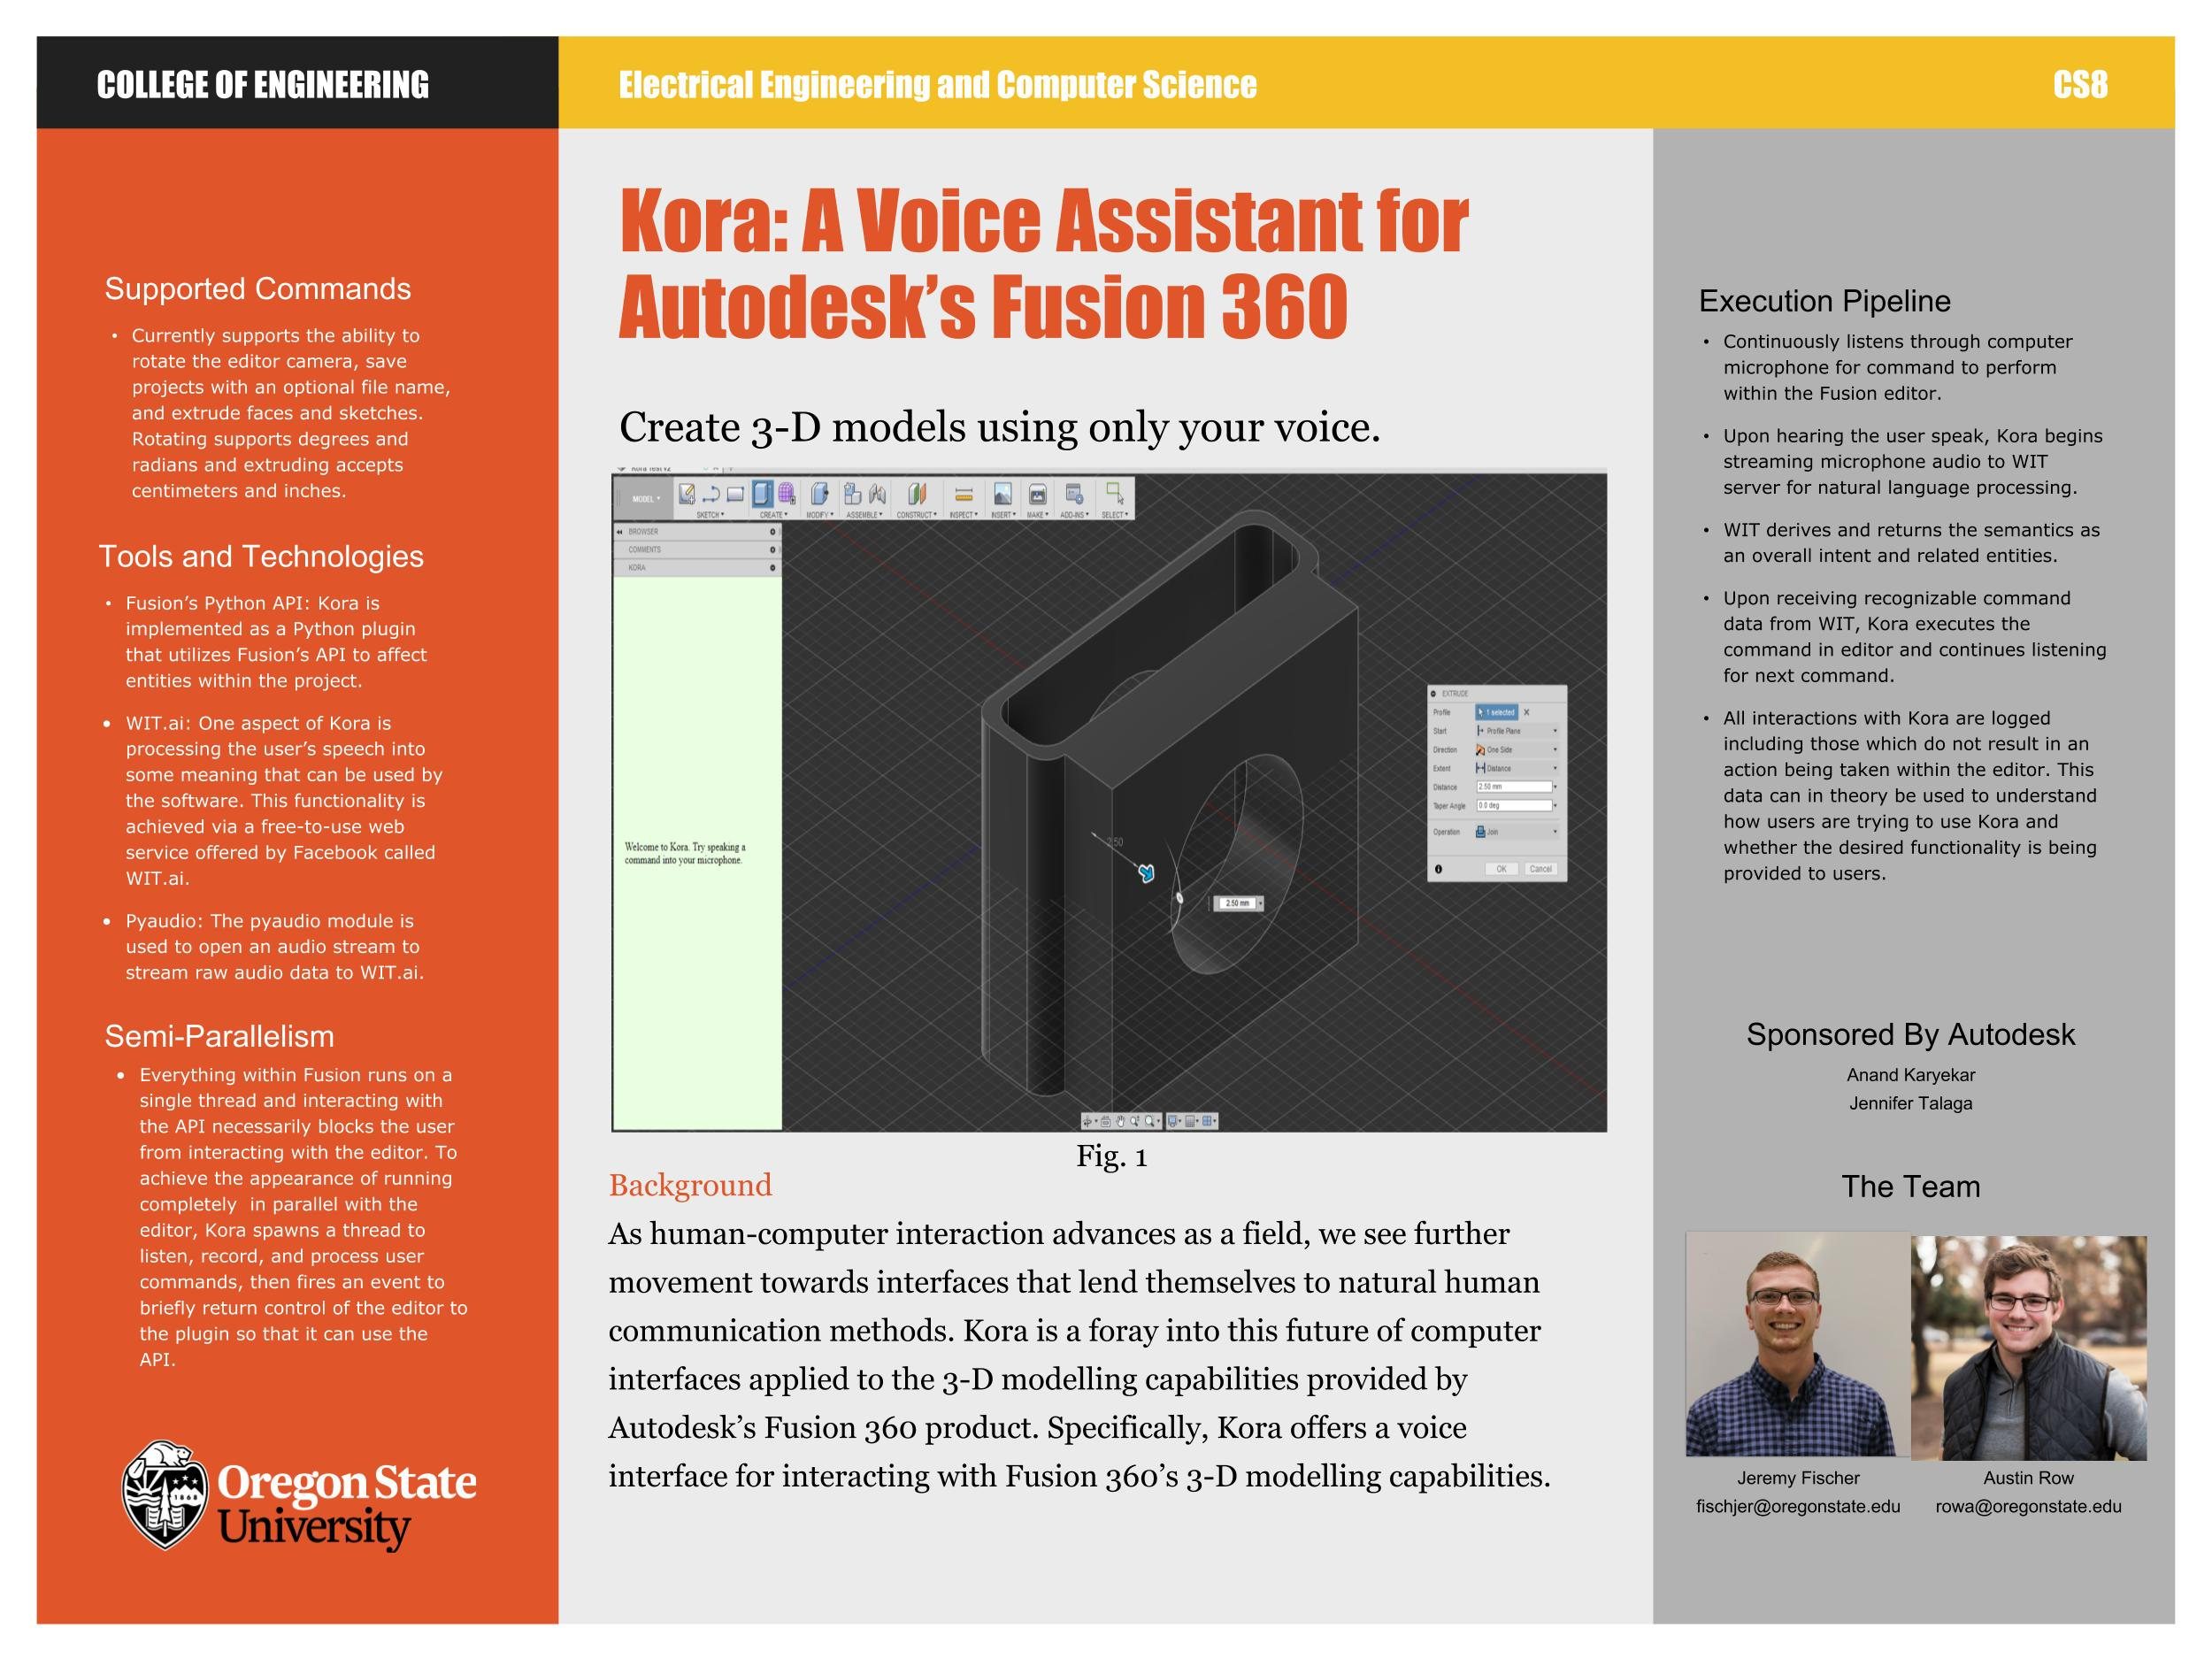
\includegraphics[width=19cm]{poster.eps}
		\centering
	\end{figure}














\section{Project Documentation}
%	How does your project work? (Could include the following...)
%	What is its structure?
%	What is its Theory of Operation?
%	Block and flow diagrams are good here.
%	How does one install your software, if any?
%	How does one run it?
%	Are there any special hardware, OS, or runtime requirements to run your software?
%	Any user guides, API documentation, etc.
%	This needs to be detailed enough to recreate and/or use your project!

\subsection{Packages}
\subsubsection{Software Needed}
Since \textit{Autodesk's Fusion 360} runs Add-Ins in their own environment, all software packages needed to run Kora had to be packaged within the Kora Add-In itself.
Lucky for you, this means the only software that needs to be install is MongoDB.
For this project we used v3.6.2, but any version newer than this will do.

A user also needs to make an account at https://wit.ai to obtain their Server Access Token.


\subsubsection{Preinstalled Packages}
The software packages that are already packaged within the Kora source code are:
	\begin{itemize}
		\item \textit{PyAudio} version 0.2.9. This is used for streaming audio from the user
		\item \textit{PortAudio}. This is an executable within PyAudio that PyAudio uses to stream audio.
		\item \textit{PyMongo} version 3.61. PyMongo is the low-level driver wrapping the MongoDB API into Python.
		\item \textit{Mongoengine} version 0.15.0. MongoEngine is a Document-Object Mapper for working with MongoDB from Python.
	\end{itemize}





\subsection{Getting Started}
Make sure you first read the Packages heading above.
	\begin{enumerate}
		\item Install Kora into the Fusion 360 Add-Ins folder.
		The Add-Ins folder is generally in

		\textbf{Windows:}
		\textit{C:/Users/<users>/AppData/Roaming/Autodesk/"Autodesk Fusion 360"/API/AddIns}

		\textbf{Mac:}
		\textit{/Users/<users>/Library/"Application Support"/Autodesk/"Autodesk Fusion 360"/API/AddIns}

		\item Name the installed repository Kora. It is important that the installed repository is named Kora, to match the Add-In name.
		\item  Go to wit.ai's website and get your \textit{Server Access Token}and paste it in \textit{Kora/main/config.py} WIT\_AI\_CLIENT\_ACCESS\_TOKEN
		\item  In Fusion click on the \textit{ADD-INS} dropdown in the top right of the ribbon, and click \textit{Scripts and Add-Ins...}
		\item  Click the \textit{Add-Ins} tab at the top
		\item Click \textit{Create}
		\item  Click \textit{Python} as the language and enter \textit{Kora}as the Add-In name
		\item  In Folder Location, browse to the Kora folder that you placed in the Add-Ins directory in step 2. Kora is now set up as an Add-In.
		\item  Open a terminal window and type \textit{mongod}to start the MongoDB daemon.
		\item  Back in Fusion, double click the \textit{Kora}Add-In, then exit the Add-Ins menu.
		\item  Click the \textit{Add-Ins} tab at the top
		\item  Click \textit{Activate Kora}

	\end{enumerate}





\subsection{Explaining The Source Code}

\subsubsection{Control Flow Diagram}
	\begin{figure}[H]
		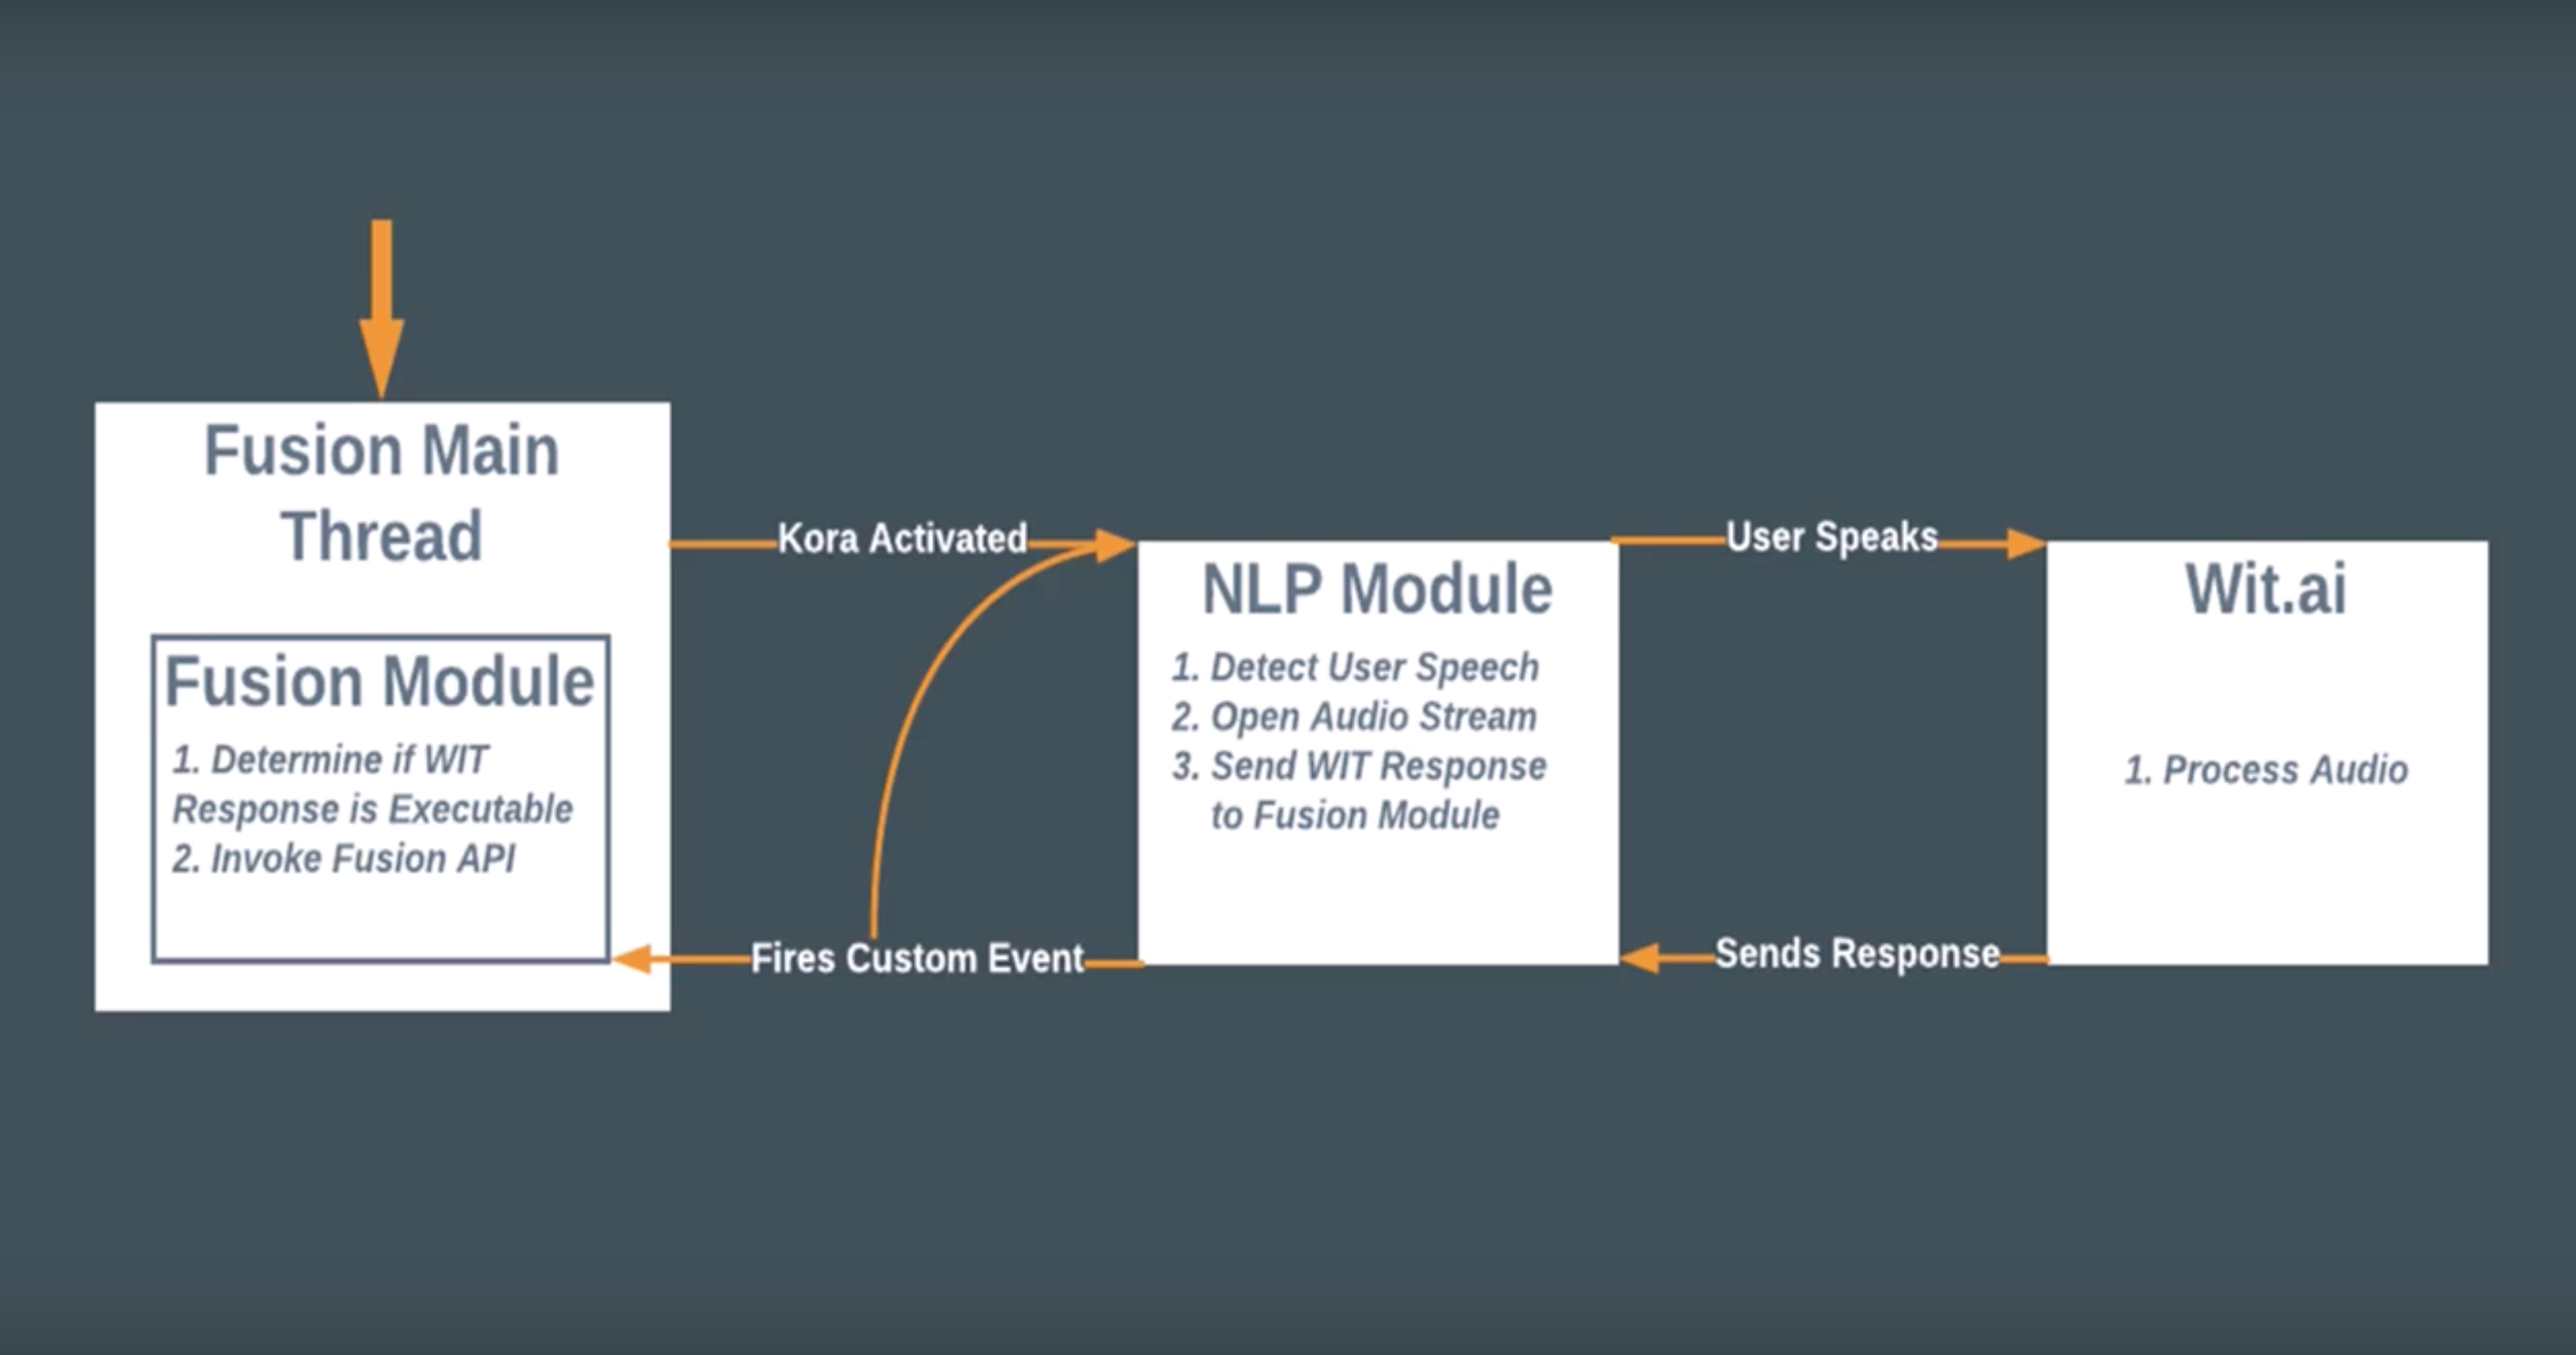
\includegraphics[width=19cm]{koraFlowChart.eps}
		\centering
		\caption{Kora's Control Flow}
	\end{figure}
The application starts in the same thread running the Fusion editor and immediately spawns a thread for recording the user voice commands and performing the natural language processing on those commands.
After a command has been parsed by WIT, the response is sent in an event that is caught and used to make the Appropriate API calls back in the main thread.

\subsubsection{User-Kora Interaction Logging }
Inside of \textit{Kora/main/modules/logging} is the relevant code.
\textbf{interaction.py} has the \textit{Mongoengine} class that outlines how the user-kora interaction document should be stored. \textbf{logInteraction.py} is the python decorator responsible for the actual storing of the interaction document. It first calls \textbf{mongoSetup.py} to initiate the connection to the mongoDB daemon.

The \textit{logInteraction} decorator is placed above the \textit{executeCommand} function in \textbf{fusion\_execute\_intent.py}. The \textit{executeCommand} function is called when Kora has a response back from Wit.ai and Kora wants to figure out what command to execute then execute it. Before that happens, the JSON containing the Wit.ai response and some extra, is routed through \textit{logInteraction}. The \textit{logInteraction} function then extracts information from the JSON then lets the JSON continue on to \textit{executeCommand}. When \textit{executeCommand} returns, it returns to \textit{logInteraction} where the remaining fields needed to store the interaction document are extracted.
Then \textit{logInteraction} inserts the interaction document into the mongoDB database.

\subsubsection{Extrude Command}
All of the commands are located in \textit{Kora/main/modules/fusion\_execute\_intent/tasks}. The \textit{extrude} function is given a string representing what the user said, the magnitude, and the units.
\textit{extrude} checks if there is a "down" in the sentence. If there is and the magnitude is currently positive, then the magnitude is changed to negative. Next, \textit{extrude} converts the \textit{magnitude} to the equivalent magnitude in terms of centimeters (the API only excepts centimeters) if the \textit{units} are not already centimeters.
Then \textit{extrude} scans through all of the profiles and faces in the project and extrudes them by \textit{magnitude} \textit{units}. If there are no profiles or faces selected, then Kora prompts the user to select the profile or face they would like extruded.

\subsubsection{Save Command}
The function \textit{save} first checks that the project has been saved before. If it hasn't then Kora prompts the user to input what they want the project to be called and then hands off the flow of control to \textit{saveAs}. If the project has been saved already, i.e. the project has a name, then \textit{save} goes ahead and saves the project.

\subsubsection{Save As Command}
The function \textit{saveAs} first checks if the call is coming from \textit{save}. If it is, then it creates a copy of the project and saves it as the supplied filename. Otherwise, \textit{saveAs} first converts the supplied filename to camelcase and then creates a copy of the file and saves it under the camelcased filename.

\subsubsection{Rotate Command}
The \textit{rotate} function begins by converting the magnitude to radians if it is not already given as radians.
The function the proceeds to determine the axis about which it should rotate the camera.
If the rotation direction is left or right, then it rotates about the vector that defines the camera's up direction.
Otherwise if rotates about a vector that is perpendicular to the camera's up direction and to the vector that defines the camera's position relative to the origin of what it is viewing, i.e. its target.
Before the rotation occurs, the axis of rotation is set to intersect the camera's target so that the camera is rotating around its target.







%	What web sites were helpful? (Listed in order of helpfulness.)
%	What, if any, reference books really helped?
%	Were there any people on campus that were really helpful?
\section{Recommended Technical Resources for Learning More}
	The entirety of the project can be completed using the following three resources:

	\begin{enumerate}
		\item \textbf{https://help.autodesk.com/view/fusion360/ENU/?guid=GUID-C1545D80-D804-4CF3-886D-9B5C54B2D7A2} \\
			Contains information regarding how to create Fusion AddIns as well as the documentation for the Fusion API.
		\item \textbf{https://wit.ai/docs} \\
			Contains the API for WIT, the web service used for handling natural language processing.
		\item \textbf{https://forums.autodesk.com/t5/fusion-360-api-and-scripts/bd-p/22} \\
			Contains the official forum for asking questions regarding building Scripts and AddIns for Fusion.
	\end{enumerate}









\section{Conclusions and Reflections}

%	What technical information did you learn?
%	What non-technical information did you learn?
%	What have you learned about project work?
%	What have you learned about project management?
%	What have you learned about working in teams?
%	If you could do it all over, what would you do differently?

\subsection{Jeremy}
	\subsubsection{Technical Information Learned}
			\begin{itemize}
				\item I expanded my knowledge of Python, such as decorators, classes, and general shorthands
				\item How to set up and run a MongoDB database locally, and how to connect to it via  Python.
				\item I learned about libraries for streaming audio, and software for extracting meaning from the audio.
			\end{itemize}




	\subsubsection{Non-technical Information Learned}
		I learned how create and deliver a presentation with confidence. Austin and I not only attended the engineering expo, but visited Autodesk's Portland location and presented our project to their staff.




	\subsubsection{Learnings About Project Work}
		\begin{itemize}
			\item I learned to always assume that a task is going to take longer than you initially think it will.
			\item I learned to communicate with your team members often.
			\item I learned to ask people who have worked on the project or similar projects for advice and guidance.
		\end{itemize}




	\subsubsection{Learnings About Project Management}
		\begin{itemize}
			\item I learned to physically take note of technical issues as soon as you  encounter them; even if you think to yourself \textit{I'll remember to come back and fix this}.
			\item I learned the importance of having a communal place where team members can send messages, and post technical issues and to-do's.
		\end{itemize}



	\subsubsection{Learnings About Working In Teams}
		\begin{itemize}
			\item I learned the importance of communicating often
			\item I learned the importance of being open to alternative ideas
			\item I learned to give credit when credit is due as well as constructive criticism
		\end{itemize}




	\subsubsection{Things I Would Do Differently If I Were To Do It All Again}
		If I were to do it all again, I would chose to use a Natural Language Processor that has built in capabilities for wake-words. Wake-words are challenging to implement well, so having that feature tied in to our NLP which we are already streaming audio to would be beneficial.
		I would also build in a testing suite earlier on, have the team commit often, and run the test suite after each push to the master. That way we wouldn't spend time figuring out and fixing subtle Mac - Windows cross-compatibility issues.





\subsection{Austin}
	\subsubsection{Technical Information Learned}
		Among the technical things that I learned while working on this project were the event-driven programming paradigm, how to use various APIs and Python libraries, and how to work with and create Python modules.
		Due to the nature Fusion 360 plugins, the implementation of the project necessarily relied on events to communicate and coordinate between various threads.
		This use of events to drive the state transitions of the application was not entirely new to me, but it was a new application of something that I have only previously been familiar with in the context of web development.
		There were also several libraries and APIs that I learned to use including the WIT and Fusion APIs and the Pyaudio library for Python.
		I had no knowledge of Python modules before this project, so I also learned how to make and use them over the course of implementing Kora.

	\subsubsection{Non-technical Information Learned}
		The primary non-technical takeaways that I had during the completion of this project were those relating to coordinating groups of people.
		This project required the coordination of multiple developers all working on different parts of the project and coordination with clients through meetings.
		I also learned to give myself a little more time than I thought I needed in time estimations since things often took longer to complete than I initially thought they would.

	\subsubsection{Learnings About Project Work}
		One of the biggest things that I have learned about working on projects is that they will likely take longer than you think they will.
		Initially, I believed that we would complete all of our main objectives early on and would be able to tackle our stretch goals before the end of Winter Term.
		This belief was naive in that it did not take into consideration the possibility of unforseen difficulties of which there were many.
		Working of this project has taught me that things will not go as smoothly as you believe and that you should take that into consideration when estimating how long it will take you to complete everything.

	\subsubsection{Learnings About Project Management}
		After approximately eight months of working on Kora, I think that the keys to project management are open and frequent communication and mutual respect amongst peers.
		We did not encounter many issues in the management of our project and I believe that it was because we had both of these things.
		Communicating ensures that everyone on the team knows what is going on and keeps anyone from accidentally doing anything in opposition to the team's goals as a result of not being informed.
		Mutual respect keeps everyone working together happily and prevents project-halting intra-team conflict.

	\subsubsection{Learnings About Working In Teams}
		I learned that while working with other developers, it is best if you can find code-related duties that are largely unrelated.
		When developers work in the same section of the code, there is likely to be conflict when you try to merge everything together.
		Having developers work on different parts of the code minimizes this risk.

	\subsubsection{Things I Would Do Differently If I Were To Do It All Again}
		If I were to do a similar project again, I would put more effort into the Technology Review.
		I was in charge of deciding what the best solution would be for handling the natural language aspects of our project, and I am not sure that I made the correct decision.
		We had significant performance issues that stemmed from our use of WIT as a web service for handling natural language processing.
		If I had put more time into the Technology Review, it is possible that we would not have been burdened with many of the issues that came from using WIT.










\clearpage


	\bibliographystyle{IEEEtran}
	\bibliography{references.bib}
\end{document}
